\documentclass[11pt,titlepage]{report}
\usepackage[a4paper,margin=1in]{geometry}
\usepackage{hyperref}
\usepackage{listings}
\usepackage{graphicx}
\usepackage{array}
\usepackage{setspace}
\usepackage{parcolumns}
\usepackage{indentfirst}
\usepackage{framed}
\usepackage{amssymb}
\usepackage{wrapfig}
\usepackage{caption}

\begin{document}

% Configurations:
\lstset{basicstyle=\ttfamily, breaklines=true}
\setlength{\parindent}{1cm}
\setlength{\parskip}{0.25cm}

% ------------------- COVER PAGE --------------------------------- %

\begin{titlepage}
% --- START Top-Right box ---
\begin{minipage}{0.5\textwidth}
\begin{flushleft}
\textbf{Faculty of Natural and\\Mathematical Sciences\\}
\small{Department of Informatics}
\end{flushleft}
\end{minipage}
% --- END Top-Right box ---
% --- START Top-Left box ---
\begin{minipage}{0.25\textwidth}
\begin{flushleft}
\scriptsize{The Strand\\Strand Campus\\London WC2R 2LS\\Telephone 020 7848 2145\\Fax 020 7848 2851}
\end{flushleft}
\end{minipage}
% --- END Top-Left box ---
% --- START kcl logo ---
\begin{minipage}{0.25\textwidth}
\begin{flushright}

\includegraphics[width=3.25cm]{img/kcl}
\end{flushright}
\end{minipage}
% --- START kcl logo ---
% --- START title ---
\begin{minipage}{\textwidth}
\vspace{1.5cm}
\begin{center}
\textbf{7CCSMPRJ \\ Individual Project Submission 2015/16}
\end{center}
\vspace{1cm}
\end{minipage}
% --- END title ---
% --- START info ---
\begin{minipage}{0.3\textwidth}
	\begin{flushleft}
		\doublespacing
		\textbf{Name:\\Student Number:\\Degree Programme:\\Project Title:\\ Supervisor:\\ Word Count:\\}
	\end{flushleft}
\end{minipage}
\begin{minipage}{0.7\textwidth}
	\begin{flushleft}
		\doublespacing
		Violetta Avkhukova \\ 1573866 \\ Advanced Software Engineering \\ Story Evolution Tracker: Tracking and Summarizing News Stories \\ Dr. Odinaldo Rodrigues \\ 14,704
	\end{flushleft}
\end{minipage}
% --- END info ---
% --- START release ---
\begin{minipage}{\textwidth}
	\vspace{1.5cm}
	\begin{framed}
		\begin{center}
			\textbf{Plagiarism Statement}
		\end{center}
		All work submitted as part of the requirements for any examination or assessment must be expressed in your own words and incorporates your own ideas and judgements. Plagiarism is the taking and using of another person’s thoughts, words, judgements, ideas, etc., as your own without any indication that they are those of another person. \\ \\
		Plagiarism is a serious examination offence. An allegation of plagiarism can result in action being taken under the \textit{B3 Misconduct Regulations}. 
	\end{framed}
\end{minipage}
\begin{flushleft}
	I acknowledge that I have read and understood the above information and that the work I am submitting is my own. 
\end{flushleft}
% --- END release ---
% --- START sign ---
\begin{minipage}{0.5\textwidth}
	\vspace{2cm}
	\begin{flushleft}
		\textbf{Signature:}
	\end{flushleft}
\end{minipage}
\begin{minipage}{0.5\textwidth}
	\vspace{2cm}
	\begin{flushleft}
		\textbf{Date:} August 26, 2016
	\end{flushleft}
\end{minipage}
% --- END sign ---
\end{titlepage}
% --------------- ABSTRACT, ACKNOWLEDGEMENTS, TOC ---------------- %
\begin{abstract}
The way people read the news is changing. Mobile applications are becoming the dominant platform for news consumption. On the other hand, people do not tend to spend a long time using these applications at one time. Additionally, news stories can have new developments as time goes on. This paper introduces the Story Evolution Tracker which aims to act as a solution to these trends. Upon article submission by the user, the system processes it through a sequence of tokenization, word importance weighing, topic word detection, and summary generation. A story is created using this information to begin tracking it for new developments, which get added to a timeline to view progression. New articles are found using the detected topic words, which the user can provide feedback for if they are or are not what they expected. The system as a whole follows a two-tier architecture, with a server doing all calculations and the user interface receiving all responses. Results of the Story Evolution Tracker are promising, with stories successfully being tracked with new, related developments. 
\end{abstract}

\renewcommand{\abstractname}{Acknowledgements}
\begin{abstract}
I would like to thank my supervisor, Dr. Odinaldo Rodrigues, for all the help, support, and advice he has given me throughout this entire project. I would also like to thank my family for the moral support and always believing in me. 
\end{abstract}

\tableofcontents
\listoffigures

% --------------------- INTRODUCTION ------------------------- %
\chapter{Introduction}
\section{Motivation}\label{se:motivation}
Reading the news is a popular way of keeping track of events in the world. In fact, 95\% of adults in Great Britain obtain the news through some media \cite{news_facts}. However, methods of reading the news are changing. Though newspapers were the main source of information in the past, most news sources now provide an online interface. As a result, 75\% of news readers obtain the information digitally. The most prominent way of reading the news is through mobile applications.  According to the Pew Research Center, 39 out of the top 50 news websites get more user traffic from mobile users than desktops \cite{digital_trends}. Interestingly, despite this trend, for only 10 out of the 50 news websites do the users spend more time in the mobile application than in the desktop version \cite{digital_trends}. 

This shift of quickly digesting the news is an interesting problem for news sources. According to the statistics, users want to read the news but do not want to spend a while doing so. A viable solution is to summarize news articles so users can get the main idea of the text without reading the entire article.

In addition, news stories can have continuous updates as developments occur. If a user has a specific interest in a topic, they would need to manually search a news website to see if there is anything new. In other cases, a news story may not be significant enough to receive breaking news notifications from the news content provider. A solution for this would be to automatically track a story's developments and view them on a timeline. The user would be able to see a clear progression of events for a specific topic they are interested in.

There are applications that perform similar tasks, but not to the same extent. The application Google News and Weather provides personalized news by tracking what topics users like \cite{googlenews}. However, it does not provide a clear picture of how a news story progresses. There is another application called Timeline, which aims to provide a historical background and progression \cite{timeline_techcrunch}, but it is curated by writers to provide history whereas in this solution, the timeline would be created automatically with new updates for specific topics the user is interested in.

\section{Aims and Objectives}
The Story Evolution Tracker will attempt to provide a solution to these problems. The aim is to create a system that will track how a user-given news story changes over time. The user will specify the URL of a news article from a pre-defined source. This becomes the basis of a \textit{story}. A story is defined as a specific, concrete topic that has one or more dedicated news articles representing its progression.

After receiving the URL, a short summary of the article, called a \textit{signature}, will be displayed to the user. A signature will be an extract of the main article. Sentences that are deemed most important will be chosen to appear in the signature. To do so, the system will perform a series of unsupervised textual analyses, i.e. no training input is given and no user intervention is necessary.

A set of automatically generated topic word labels will also be shown so the user can quickly identify the main topics that are tracked by the system. These topic words will be used to retrieve new developments. 

Each story will have a \textit{timeline} associated with it. A timeline is defined as a sequence of signatures with timestamps to show what events have occurred for a specific story. New articles will be added to the timeline automatically when new developments are available. Additionally, the user will be able to provide feedback on the newly retrieved article based on whether it matches what they wish to read about.

The main areas of investigation for this project will be getting news articles from the Internet, processing the article's text to get useful information, summarizing the article to get a signature, retrieving more articles related to a news story, and displaying all this information to a user.

\section{Report Structure}
The rest of this report will be structured into chapters, each one focusing on a different aspect of the Story Evolution Tracker. Chapter 2 will explore a theoretical background relating to the main areas of investigation. Chapter 3 will go into the specifications and design that will shape how the software comes together. Chapter 4 will explain the implementation and various decisions that were made during that process. Chapter 5 will go into the testing and evaluation of the software to see whether it performs as required. Chapter 6 will go over conclusions and the potential for future work.


% ------------------------- BACKGROUND ----------------------- %
\chapter{Background Review}
\section{Overview}
The previous section introduced the motivation and aims relating to the problems given. In this section, previous work in the main areas of investigation will be examined and evaluated in relation to the goals of this project.
\section{Topic word detection}
There has been extensive work done in detecting a set of topic words, or keywords, for a given text. Keywords are defined by Rose, Engel, Cramer, and Cowley as “a compact representation of a document’s content \cite{RAKE}. Another reason they are useful is because each keyword can serve as part of a query during information retrieval \cite{RAKE}.
\subsection{Statistical and linguistic analysis}
The first work investigated is an approach by Gupta, Dixit, and Sharma \cite{gupta}. They have developed an unsupervised algorithm of detecting topic words, so there is no training by the system. A set of statistical strategies are used to rank words based on various criteria. Their goal is to summarize web content in this style by generating a set of keywords. First a set of text processing steps occur, which includes tokenization, stemming, and stop-word removal. After this, words are scored based on a statistical and linguistic analysis of the text. Words are weighed based on their appearance in sections like the title of the text, the URL, and if the word is highlighted in the text at any point. Also considered is the part-of-speech and range covered by the word in the text, i.e. where it appears first and last. The score is computed after taking all of this into account. The top N highest-scoring words are selected to be the topic words \cite{gupta}. 
\subsection{Local and global recurrence measure}
Another method was introduced by Chi, Chen, Su, and Shi \cite{sushi}. They mention the popularity of using features of the text, like the title, word position, and part of speech, as part of a word weighing scheme. They also closely examine another measure called local reoccurrence (LR), which determines highly ranking words by seeing how frequently they occur within their local area. The motivation behind this is that common, unimportant phrases may still occur frequently, but they would be spread around, so their LR score will be low. A downside of this method is that some words may be incorrectly flagged as important in a section of a text where they occur a few times but do not appear anywhere else. Chi, Chen, Su, and Shi have proposed another method called global reoccurrence (GR) measure to compensate for these downsides \cite{sushi}. They introduced the concepts of lone clusters and non-lone clusters to clarify the occurrences of a phrase. Lone-clusters are a single occurrence of a phrase and non-lone clusters are several occurrences of a phrase within close proximity. A higher GR value is given to a phrase that has a higher frequency of non-lone clusters. Common phrases occur throughout the whole text, but because they tend to not repeat multiple times within close proximity, a low GR value is given. Another approach they give is the C-value, which gives higher importance to words that are not nested within others; a keyword is more preferable if it not nested inside another.. Keywords are determined by considering the highest GR values and C-values \cite{sushi}.
\subsection{Rapid Automatic Keyword Extraction}
A method called Rapid Automatic Keyword Extraction (RAKE) was introduced by Rose, Engel, Cramer, and Cowley, which extracts keywords for a single document, regardless of other documents, domain, or type \cite{RAKE}. They make the assumption that keywords do not generally contain any punctuation or stop-words but can be composed of multiple words. Stop-words are considered to be uninformative, so as in the previous works, they are dropped from the text. Word that remain are called context words. RAKE takes three parameters: a list of stop-words, and delimiters for both words and sentences. First, the text is parsed into individual words, followed by separating the words into sentences. For each word, a score is calculated for each of its member words considering three calculations: word frequency, word degree (which gives more importance to words that occur frequently and inside longer candidate keywords), and the ratio of degree to frequency. They also included support for words that contain stop-words within them, e.g. “degrees of freedom”. Keywords that are joined by a stop-word at least twice in the same order are included into the list of candidate keywords. Since these types of words do not occur as frequently as normal words, their importance is higher because of their rarity. After finishing the rankings, the top N words are selected to be the keywords best representing the given text \cite{RAKE}.
\subsection{Analysis}
The three methods investigated above provide insight on how keyword extraction can be performed. All three methods consider aspects of the text like how to tokenize the words into individual entities, the removal of stop-words, performing a ranking of some kind using numeric values, and taking the top N words. The first two methods, as proposed by Gupta, Dixit, and Sharma and Chi, Chen, Su, and Shi perform analysis on the text like part-of-speech tagging and various location-based weighing. Notably, weighing on the spread of a specific word is an interesting metric of how important a word can be. However, in the case of news articles, where the content follows a “top-heavy, inverse-pyramidal structure” \cite{zhao}, methods of word spread may incorrectly devalue the importance of words which only appear in the beginning of news articles. On the other hand, using the technique of weighing certain parts of the text higher than others may prove useful for news articles. The RAKE system does well to consider the relationship between a word’s frequency and the context it appears within, as well as support for keywords that contain a stop-word. However, it seems to favour keywords that are composed of at least two words because it looks for word co-occurrences. This could prove to be an issue if a news article is consistently about a single-word keyword. Overall, these works explain very well the many ways keywords can be extracted.
\section{Text Summarization}
The need for text summarization is growing due to the amount of texts available on the Internet. To save time, a shorter version of texts can be given to a user while still capturing the main ideas.
\subsection{Rule reduction}
The first work investigated is by Devasena and Hemalatha, where a system of rule reductions is used to make text more concise \cite{devasena}. First, the given text is tokenized into words, whitespace, and punctiation. Next, each word is labelled with its part-of-speech, such as a determiner or verb. Then using a set of rules, the words are grouped into noun phrases, verb phrases, and the like. Using these sentence components, several can be eliminated to provide a shorter summary \cite{devasena}.
\subsection{HedgeTrimmer}
HedgeTrimmer, developed by Dorr, Zajic, and Schwartz, is a system that generates a headline using the first sentence of a news article \cite{hedgetrimmer}. The goal is to create a concise version of the main topic of the article, without losing any important details. They use only the first sentence of the news article because they discovered that 86.8\% of words that are in the headline appear in the first sentence of the news story. Their approach first parses the text into a parse tree of nested noun phrases, verb phrases, et cetera. Afterwards, a process of trimming the sentence begins by choosing the first noun-phrase, verb-phrase combination and removing units such as time, determiners, and unnecessary prepositional phrases and sentence clauses. What is left is a concise headline-style summary of the first sentence, giving a brief overview of the article’s contents \cite{hedgetrimmer}.
\subsection{Information retrieval techniques}
An approach proposed by Gong and Liu for summarization involves standard information retrieval methods to choose the most relevant sentences from the text. Their main goal is to produce summaries out of sentences that are important but cover different concepts. They define a generic summary as one that covers “the main topics of the document” and “keeps redundancy to a minimum” \cite{gong}. The first step is to tokenize the text into sentences. Next, a weighted term-frequency vector is created for each individual sentence, which depends on local and global weighting for each term. However, any type of weighting scheme can be used. The main aspect of their summarization approach is choosing the highest weighted sentence, adding it to the summary, and then removing it and its terms from the text \cite{gong}. This ensures that each next sentence that is added to the summary has a different main topic, guaranteeing the least amount of redundancy.
\subsection{Analysis}
The above methods give different strategies on how to achieve various types of summaries. The method of rule reductions proposed by Devasena and Hemalatha is a novel approach of doing iterative shortening of some text. However, it relies too heavily on perfect grammatical structure. Even if the grammar is correct, sentences can be more complex than defined by the rules due to the non-deterministic nature of language. The HedgeTrimmer method by Dorr, Zajic, and Schwartz improves on this by flexibly deciding which parts of the sentence can be eliminated by looking for unnecessary sentence constructs. Although this is useful for making a summary shorter, using only the first sentence to summarize an article may be inadequate. Additionally, if a summary of one or two sentences is obtained by other means, this type of iterative shortening may be unnecessary after all. Finally, in the case of the work done by Gong and Liu, their algorithm does a good job of getting a spread of information from any given text. However, in the case of news articles, where each story is focused on a specific topic, there may not be many sentences to choose from on each iteration of the algorithm. There is a risk of a lack of cohesion if a sentence that is not the main focus of the article is chosen. This algorithm may be more suited for longer texts, whereas most news articles tend to not be overly long. 


% ------------------------- SPECS & DESIGN ----------------------- %
\chapter{Specification and Design}
\section{Specification}
\subsection{Overview}
The specification explains what the software will need to do in order to meet the aims and objectives. This is explained in terms of requirements for each of the main areas of investigation involved. 
\subsection{Retrieving articles from the Internet}
The first step is to retrieve the article that the user specifies from the Internet. The system must provide an interface for the user to input a URL for a web page, which should contain a news article. The software will then perform validity checks to see whether the given URL fits the pattern of the allowed sources. The software will only support articles found on the British Broadcasting Corporation (BBC), although support for additional news sources should not be difficult to add. If the URL is deemed to not fit any of the accepted sources, the system should exit elegantly with a clear error message. If the URL matches one of the accepted sources, the system should retrieve the contents located at the URL.  

The system must extract only the useful information from the web page to process. This includes the headline, the article's timestamp representing the date published, and the article body. If one of the required elements of the article is not found, the system must exit gracefully with an error message. Once these steps are completed, the process of retrieving articles from the Internet is completed. The data retrieved should be stored in a format that is simple to use and access, as it will be vital during the next processing steps.

\subsection{Processing an article's text}
The goal of processing the text is to extract useful information. One important feature is determining a set of topic words that accurately represent the contents of the text.

First, the article text must be tokenized into words and sentences. The text includes all features representing the main information of the news story, such as the headline and main article body. No information should be eliminated during the tokenization process, including punctuation. The tokenized text must be stored in a convenient format because of its importance for the subsequent processing operations. 

Next, for each unique word in the article, its importance must be determined. Importance is a measure of how well a word represents the main topic of the news story. Importance should be determined by a number of factors, one of which is to be based on the word's location in the article. For instance, a word that exists in the headline must be given greater importance. Proper nouns, such as people or places, must be given more importance. The exact values are to be determined. Other techniques should consider the article formatting that exists for a specific news source, like any sections that are consistently bolded in mark-up. 

Once each word has an importance value assigned, at least five topic words must be chosen. Each chosen topic word must be a noun, either singular or plural, or a proper noun. No dates, adjectives, or numbers on their own should be a topic word because they do not add any value when taken out of context. In addition, topic words must be specific enough that they can be used in a query to find similar articles.

\subsection{Summarizing the article}
Once words are weighed, the article must be summarized to create the signature. The signature is to be an extract of the main article. That is, some number of sentences that are deemed the most important will become the signature. Here, a requirement of at least two sentences is set for articles that are at least two sentences long. Otherwise, the article is one sentence long, which becomes the signature.

To choose the important sentences, the system should consider the word importance values that were generated in the previous step. This is because the sentences with the higher weighted words should be considered more important because they more accurately cover the main idea of the article.

The top sentences will be the signature. There must be an effort to shorten the signature of any unnecessary words or clauses. The sentences of the signature must be in the same chronological order they appear in the original article. The signature of the article is the main element that will be displayed to the user. The quality of the signature must be high. Attributes of a high quality signature include sentences that make sense when taken out of context, sentences that are related to the topic words, and at least one sentence must capture the main essence of the article.

\subsection{Retrieving new articles}
For each story the user is tracking, the system must retrieve new articles that are related to the story's topic. New articles must be found on the BBC website due to the intended support for BBC articles.

Articles should be weighed based on similarity to the tracked story. The news article with the highest similarity would represent the next article that is added to a tracked story's timeline. 

News article similarity is defined as how closely the articles in comparison represent the same topic. A variety of schemes can be used to measure similarity, which is to be investigated during implementation.

If an article is found with a similarity high enough to be related, it must be added to the front of the tracked story's timeline. The new article's URL, timestamp, headline, topic words, and signature are the minimum information that must be given to the user. If an article is not found or no article was determined to be similar, the system must send a response saying that there was no update to the story.

This aspect of the system is a crucial step in order to track a story's progression. The user must be able to send a request to update his or her tracked stories at any time.

\subsection{Displaying information to the user}
The user must have access to a user interface to perform operations related to tracking stories. The user must have a main screen that displays all stories that the user is tracking. If there are no stories tracked, the screen should say so. Otherwise, each story must be easily identifiable so the user remembers what is being tracked. 

The user must be able to view the timeline of each story. The timeline must clearly portray the story's sequence of events, such that the most recent development is seen first. For each development shown in the timeline, the user must see at least the signature and timestamp for that entry. When a new development comes in, the user should receive a notification stating that there is an update to view.

Additionally, the user must have the option of providing feedback. Feedback will go towards articles that are automatically retrieved for a story. Positive feedback would imply that the user approves of the article that was picked for them, i.e. the newly chosen article is indeed an accurate development of the story. Positive feedback strengthens the topics that the user wants to hear more about. Negative feedback would imply that the article chosen was not a good fit for the tracked story or it is something that the user does not want to read about. The feedback can be used to imply the user's interests. 

In terms of story management, the user should be able to delete tracked stories from their profile when they no longer wish to see updates for a topic or there have not been any new developments for a while. Adding new stories should also be simple to do. 

Other requirements include validity checking on any user input fields so that any incorrect input will not crash the system. User data must be persistent so the user can come back to view their tracked stories. 

\section{Design}
\subsection{Overview}
This section will talk about the different ways the system can be structured considering the requirements. Each design consideration will be weighed in terms of advantages and disadvantages and a best potential design will be chosen.
\subsection{Initial design considerations}
Considering the requirements stated above, there is a clear divide between a user front-end and a processing back-end. The front-end would involve all operations a user can perform, like viewing all information relating to their tracked stories. The back-end would perform all text processing, signature generation, and new article retrieval. Although it is technically possible to perform every user and processing operation on a single tier, performance may suffer due to too much happening on a single thread. Multi-threading could be introduced, but some languages do not have support for that. Therefore, it is best to separate the user front-end and the processing back-end into two tiers. 

Another consideration is which programming language to use. There are many to choose from, such as Java, C++, JavaScript, and many more. Each one has it advantages and disadvantages when it comes to ease of use, support for external libraries, and structuring of components. Also, because of the divide between the front-end and back-end, different languages can be used for each. One deciding factor when choosing a language is the nature of the content that will be worked on. 

For the article processing back-end, the user would submit a URL to a web page. A natural fit for working with web content is JavaScript. JavaScript is a language that is best known for web page scripting and development, although it can be used in non-web environments as well \cite{javascript_info}. It has a lot of support for web code manipulation through its extensive collection of libraries. Because of these qualities and the fact that the user process web pages for their content, JavaScript may be a natural choice. 

Other language choices include Java, which also has support for web requests and web page manipulation through external libraries. However, some downsides include the overhead that comes with Java and the Java virtual machine that the compiled code runs on. Comparing this to JavaScript, which is lightweight and runs straight on the browser or server, this is an overhead that can be avoided. Another downside to Java is the rigidity of variable and object instantiation. JavaScript allows a lot of freedom when it comes to assigning values to variables as it is loosely typed. JavaScript allows for the use of simple JSON-style objects, which are similar to maps with key, value pairs. Attributes can be added and removed at any time, which makes data storage very simple. Also, due to the web requests that need to be made for retrieving article information, JavaScript naturally handles asynchronicity through the use of callbacks which are called once an operation is complete. Having considered all these factors for the back-end, JavaScript is a clear winner when it comes to data manipulation involving web content. The user front-end can be built for any platform, such as web or mobile applications. It can communicate with the back-end to perform an operation and then show the result to the user after receiving the response.

Another design consideration is how to structure the code. Based on the requirements above, there seems to be a modular pattern to the steps involved. Each of the requirement areas listed can become its own component since they all represent unique processing steps. An advantage this brings is that each can be developed individually and there is a separation of concerns which aids organization and understandability. Additionally, if one of the modules would need to be improved, they can be swapped for a different implementation, as long as it still takes the same argument parameters and returns the same output format. A disadvantage is that more files would need to be managed if each component is separated into its own file, but the advantages outweigh the disadvantages. As a result, the best course of action is to have a module for each of the steps listed in the requirements.

\subsection{Article HTML extraction and parsing}
This is the first module that will initiate the article processing steps once the user submits a URL. This will run on the back-end. Retrieving the URL is a concern for the user interface, which passes it to this module. First, a set of validity checks should take place. Validity checks include to see whether the input is a URL, if it is blank, and if the URL matches the allowed news sources. This can take place on either the front-end or back-end. An advantage for the case of the front-end is that it is fast since no requests are made, but it may complicate the user interface code which should be responsible for receiving and showing data and the checks may need to be re-written in multiple user interfaces if there is more than one. In the case of the back-end, the front-end would need to make a request to see if the URL matches any of the allowed news sources. This can be slow because it would need to send a request over the Internet and wait for a verdict. Instead, a combination of these steps can be used. Any user-interface specific checks, such as checking of the input field is empty or does not conform to a URL pattern can be done on the client side. If it passes those simpler checks, the server can then do its own validity checks to see if the URL pattern matches the allowed sources.

The next step is to retrieve the contents located at that URL. This can be done in the most obvious way, which is using HTTP GET requests. Once a response containing the page contents is received, the HTML code can be processed. The goal of the processing is to extract all information relating to the article. Each news source follows a pattern when it comes to formatting their news articles which does not tend to change. Because of this, each element of the page that contains article information can always be referred to by the same id or class. For instance, the headline of an article will have a unique id or class by which it can be referred to. Additional news sources can be configured if their article formatting styles are examined. It is important to consider the ease of adding new configurations for additional news sources. The design should be as modular as possible as to minimally affect core functionality files, so in other words, configurations for all sources should be separated from the main text processing functionality. This helps when existing configurations must be changed because core files would not be altered, only a configuration file.

Another important consideration for this module is dealing with articles that do not have the expected structure for that source. When looking for a specific id or class representing a part of an article and it does not exist, it may mean that this article is not suitable for parsing and tracking. This is because some information is missing to create a high quality signature. Although a news source can contain several configurations for extracting information from articles, there are many pages on the news source's website that are not articles that pass through the URL validity checks.

This module must send a response that contains the headline, article body, and timestamp. It will serve as input for the next step in the article processing chain.

\subsection{Text processing}
This module will be involved with calculating the importance of words and detecting a group of topic words that represent the main concepts of the article. It receives as input the parsed article from the previous module.

Its first responsibility is to tokenize the article's text. There can be several ways of doing this. In JavaScript, there is a global string method called ``split'' which acts on the invoking string and returns an array of words after separating the string on the given argument. A common argument is a space character so a sentence is split on all spaces. This technique is good for words that are not adjacent to punctuation, otherwise the punctuation is considered part of the word since there is no space between the two. To have a high-quality tokenization, all punctuation should remain because no information is to be discarded at this early stage. The difficulty of this approach starts increasing if to consider all possible punctuation. Another method is to use an external library that specializes in tokenization. After all, tokenizing can be considered an intermediate step that functions like a utility.

Representing the tokens can be done in several ways. One idea is to have each sentence to be an array, where each index is either a word or punctuation. No white-space is stored as it is implicit based on the splits and adjacent punctuation. The article can be represented as an array of these sentence arrays. This should be stored as additional information, i.e. no information must be overwritten from the previous module. 

The next step is calculating word importance. There can be many different techniques involved here. One way is to use term frequency-inverse document frequency (tf-idf). Words that appear too frequently would be given a low tf-idf because they appear many times in many documents. Words that appear frequently but in only some documents may be given a higher tf-idf, although it depends on the document corpus \cite{torres}. A score can be assigned to each word based on this algorithm, although it can lose meaning if only doing it on one document since each result depends on a corpus.

Another potential method is simply calculating word frequency. It can be a good indicator of word importance and it is also a method of determining all unique words in a text. Although, it is important to remember that common words will also rank highly.

This brings stop-word identification into account. Words that are just sentence utility words, such as ``the'' and ``a'', should not be weighed because they do not add any value. This is similar to detecting word part-of-speech. Nouns are preferred as topic words because they define concepts, whereas adjectives and adverbs describe concepts and add no value when taken out of context. Similarly, another class of words to detect is proper nouns, which can be better candidates for topic words since they are a stronger type of concept, like a person or place. One quality that may be considered for detection is if the word is capitalized or not throughout the whole text.

A numeric score can be assigned to each word for ranking. If the words are sorted in descending order of score, the top N words can be chosen to be the topic words. As stated in the requirements, topic words should only be nouns, whether singular, plural, or proper. Since the words were sorted in descending order, the first topic word is the most relevant, the second word is the second most relevant, and so on. 

This module should send a response containing all the word weights and topic words because they will be useful for the subsequent modules.

\subsection{Signature generation}
This is the last module that would get run when given a URL by a user. It uses the response from the previous module to rank sentences based on the word importance values. 

One method that would be simple to implement is calculating the sum of all word values for each sentence. The sum would become the importance of the sentence. Once this is done for all sentences, they can be sorted in descending order of importance. The top two or more sentences are chosen to be part of the signature, which are added in chronological order. 

A downside to this method is that the longest sentences may end up with the highest scores, regardless of how important the composing words are. One method could be to penalize sentences based on their length, such as dividing the importance by its word length to become its final importance value. Other techniques can be investigated during implementation.

Another technique to consider is shortening the signature. Clauses such as ``According to'' or ``said researchers'' can be removed because they do not add much value. The signature should be as to-the-point as possible. Removing unnecessary adjectives or black-list words, such as ``the'', can also shorten the signature. In addition, this module can also improve readability of the signature by replacing pronouns with the names of people being referred to. 

The response of this module must contain the signature in a plain text format as it will be displayed in the user interface. If shortening techniques were used, the plain text versions of the sentences from the original article cannot be used. The sentence array would need to have its words concatenated into a correctly-formatted sentence, taking care to make sure all punctuation looks correct.

\subsection{Retrieving new updates}
The goal of this module is to find new developments for a tracked story. The first thing to decide is where to search for new articles. In general, it must be some place where parsing articles for that news source is supported. Because the BBC is a requirement for the Story Evolution Tracker, one idea is to take advantage of their searching algorithm and use it as the engine for new articles. To use this method, the search criteria must be decided on. Generally, the system must find articles that are related to the tracked story.

One idea is to send all the topic words of a tracked story as part of the request for an update. Some number of words taken from the front of the topic words list can act as part of the search criteria. The number of words to use is to be decided. One word may be too general of a search criteria, two words may be a good amount, and three words may provide the specific search criteria but it may start restricting the search results too much. The best case of action is likely using two words because it is better to show the user some article even if it is not an exact match because the user can provide negative feedback on that article.

If following this approach, it means doing an HTTP GET request to retrieve the search results from the BBC's search page since they do not provide a public searching API. This page would need to be parsed in a similar way as news articles to get each individual result. First potential matches need to be found among these, then an HTTP GET request needs to be made for each result to retrieve the topic words and signature.

There can be several ways of determining potential matches. One way is to use all search results as potential matches to be the next development. Another way is to check if any of the topic words from the tracked story appear in the headlines. There are advantages and disadvantages to both approaches. The first method is simple to implement but it may be a waste of time parsing some of the search results as they may not be related. The second method will save on performance but headlines are not guaranteed to be descriptive of the article's main topic. The best course of action is to use the second method because it will save on performance and it will not be at risk of getting potentially off-topic articles. In addition, filtering on the timestamp can save on some performance because articles that are older than the most recent development are not new developments. Once this is done, the text processing of each article begins.

The next step is to rank articles based on relatedness to the tracked story. The top ranking article should be chosen as the new development. One idea for this is to compute a similarity score for each article to see how it compares to the original story. Many different techniques can be used. One way is to compare how many topic words overlap between the tracked story and the current article. Another way is to assign points for topic word matches; for every match, if the positions of the topic words are the same in their respective arrays, then the most amount of points can be added, otherwise fewer points are added. The latter is likely to be a better method because it will consider strong topic word matches. For instance, if the same topic word is in the first slot for both arrays, a lot of points are assigned because both are strongly about that word. 

Article similarity should have a threshold to exceed. If it goes over the threshold, article with the highest score is the new development that is appended to the story's timeline. At least the signature, headline, topic words, and timestamp of the new article must be sent in the response. If there is no article found or no article over the similarity threshold, the user should simply not be updated. 

Using this approach, a new story can be found. This design can be altered with by various formulas for calculating similarity points and the threshold. This approach also raises the question of future expansion as new sources are supported. As the BBC is the only expected source at the moment, it is simple to use the BBC website to search for new articles. Once new websites are supported, it would be unreasonable to perform a search criteria on each news source due to performance reasons. One way to fix this is by investigating real web crawlers that are available and filter based on supported sources. This way only one request would be made to find new articles instead of one for each supported source.

\subsection{User Interface}\label{design:ui}
The user interface is an important part of the system. The requirements state the user must see all their stories, timeline, and all information associated with them.

One potential interface can be a mobile application. Android, a popular mobile platform, is a good candidate for development because it is free and openly available for development. It also fits the trends that are seen in statistics of people using news applications more than desktop but not wanting to spend a lot of time doing so nevertheless.

The application can have a screen for tracked stories. When clicking on a story, the user would be able to see the timeline of events. The timeline can be viewed either vertically or horizontally, but the first visible entry should be the most recent. There can also be a screen where the user can delete tracked stories when no longer interested. The application can communicate with the back-end server to retrieve updates and send notifications when there is something new to read. There are many ways in which this application can be developed so the user has the most quick and satisfying experience.

Another possibility is a web application to display data. A similar style can be developed for the website, but based on the statistics, a mobile application is best suited. 

% ------------------------- IMPLEMENTATION ----------------------- %
\chapter{Implementation}
This chapter will explain the implementation of the Story Evolution Tracker, taking into account the requirements and design considerations.
\section{Server construction}
The first implementation decision is choosing the programming language. Having considered the advantages and disadvantages of several languages, the best suited one for the back-end is JavaScript. It is the best choice because of the simplicity of the programming environment and ease of adding support from external libraries if required. 

Since JavaScript is normally for a client-side browser environment and the goal is to have the text processing on the back-end, a JavaScript solution for that environment is needed. Fortunately, there is a popular JavaScript back-end framework called Node.JS. It is described as an ``asynchronous event driven JavaScript runtime'' that builds server-side ``scalable network applications'' \cite{node_js}. It has support for thousands of libraries through node package manager (npm), which makes code modular and flexible. Their main premise is that by using small building blocks that are available through npm, developers can focus on their task at hand \cite{npm_about}.

Another aspect of the back-end server is considering how to make requests to perform some task, such as generating a signature for an article. A standard way is to send GET or POST requests to some URL with a request body containing information needed to fulfil it. With this in mind, an application layer is needed to respond to these requests. There is popular framework for developing web applications on Node.JS called Express. Express is an open-source lightweight application server by providing a ``robust set of features for web and mobile applications''; it makes it easy making an API for many HTTP methods \cite{express_js}. Node.JS and Express are often used together when this type of functionality is needed.

This pattern is exactly what is done for the back-end of the Story Evolution Tracker. The \lstinline|index.js| file in the project contains all routes that the server can respond to. A route is an extension of the URL that identifies a resource in the server. For instance, in \lstinline|http://localhost:3000/process_article|, the part  \lstinline|/process_article| is the route that would get invoked by the application server. It gets invoked when the specified HTTP method is called for it. As an example, the following code would run if the route specified was \lstinline|/process_article| and the HTTP method received was POST:
\begin{lstlisting}
   router.post('/process_article', function (request, response) {
  	   // this code executes when received POST request with route /process_article
   });
\end{lstlisting}
The \lstinline|request| parameter contains all information about the request, including the body that holds information given by the user interface. The \lstinline|response| will get information added onto it about the content type, response code, and response body containing the result of the user's request. Invoking the send operation on the response completes the request. In this project, the responses are always in JSON (JavaScript Object Notation).

With these basics implemented, any web or mobile application can send a request to the server to perform an operation. At least two operations are obvious candidates for their own route: processing a single article to generate topic words and a signature and requesting an update for an existing tracked story.

\section{Article HTML Extraction and Parsing}
This is the first module that initiates processing of a user given article. It receives a URL from the application layer that was passed in through the request body from the user interface. The main functionality of this module is implemented in the \lstinline|htmlParser.js| file. 
\subsection{Getting URL's contents}
Using the given URL, a GET request is made to retrieve the article's contents. Node.JS has native support for this through its HTTP module. It is also asynchronous, so once the response ends, the corresponding callback is called with the entire response. 

There is also support in this project for locally stored news articles. If the URL is preceded by the \lstinline|file://| protocol instead of \lstinline|http://|, then it is loaded from local disk. The saved news article, which is either an \lstinline|html| or \lstinline|htm| file, must contain the original URL at the top of the file. This method is supported for Google Chrome's saving procedure. The reason for having locally stored news articles is so that the later text processing algorithms can be compared during development without the article being changed by the BBC.
\subsection{Extracting article information}
First the source of the article must be checked by looking at parts of the URL. It will decide the parser that will be used for that page. If the URL does not match any of the supported sources, an error message will be sent saying the cause. Otherwise, parsing will continue with the specified parser. Originally, there was support for only one article format and it was written directly in the \lstinline|htmlParser.js| file. However, to make it more modular, the file \lstinline|parsers.js| was created. It currently contains support for two different sources: BBC News and BBC Sport. Even though both are by the same news agency, they are formatted differently. In the future, more parser configurations can be added to this file or more parser files can be created. For instance, there can be one for each source with multiple configurations per source. 

Next is extracting data. In the first attempts to parse web pages, jQuery was to be used. It is a well-known client-side DOM-tree parsing library. However, to use it, a browser environment had to be emulated. It ended up complicating the code too much because of many nested functions and a lot of overhead, so a re-evaluation was needed. Instead, the system now uses a library called ``cheerio'', found in the node package manager. It functions very similarly to jQuery but it is natively built for Node.JS. The article's HTML code is loaded into cheerio and using CSS-style selectors, individual parts of the page can be extracted \cite{cheerio}.

For example, looking at a BBC article of the standard variety (not live, gallery, or video), the main elements to extract are the headline, date, section, and article body. The headline has the class \lstinline|.story-body__h1|, so getting its text gives the headline. Similarly, the timestamp (in seconds) is extracted by looking at the \lstinline|.date| class's attribute \lstinline|data-seconds|. The story body is contained inside a \lstinline|div| with the class \lstinline|.story-body|. Extracting the text of all \lstinline|<p>| elements gives the paragraphs of the article. The bolded sentence at the front of BBC articles is also extracted separately. If article information like the headline, date, or body are missing, the article must be of a different style and is likely not suitable for parsing. An error is thrown to the user interface saying the article has an invalid format. Refer to Figure \ref{fig:bbcArticle} on page \pageref{fig:bbcArticle} for an example of which fields must be retrieved for BBC News articles.

\begin{figure}
	\centering
	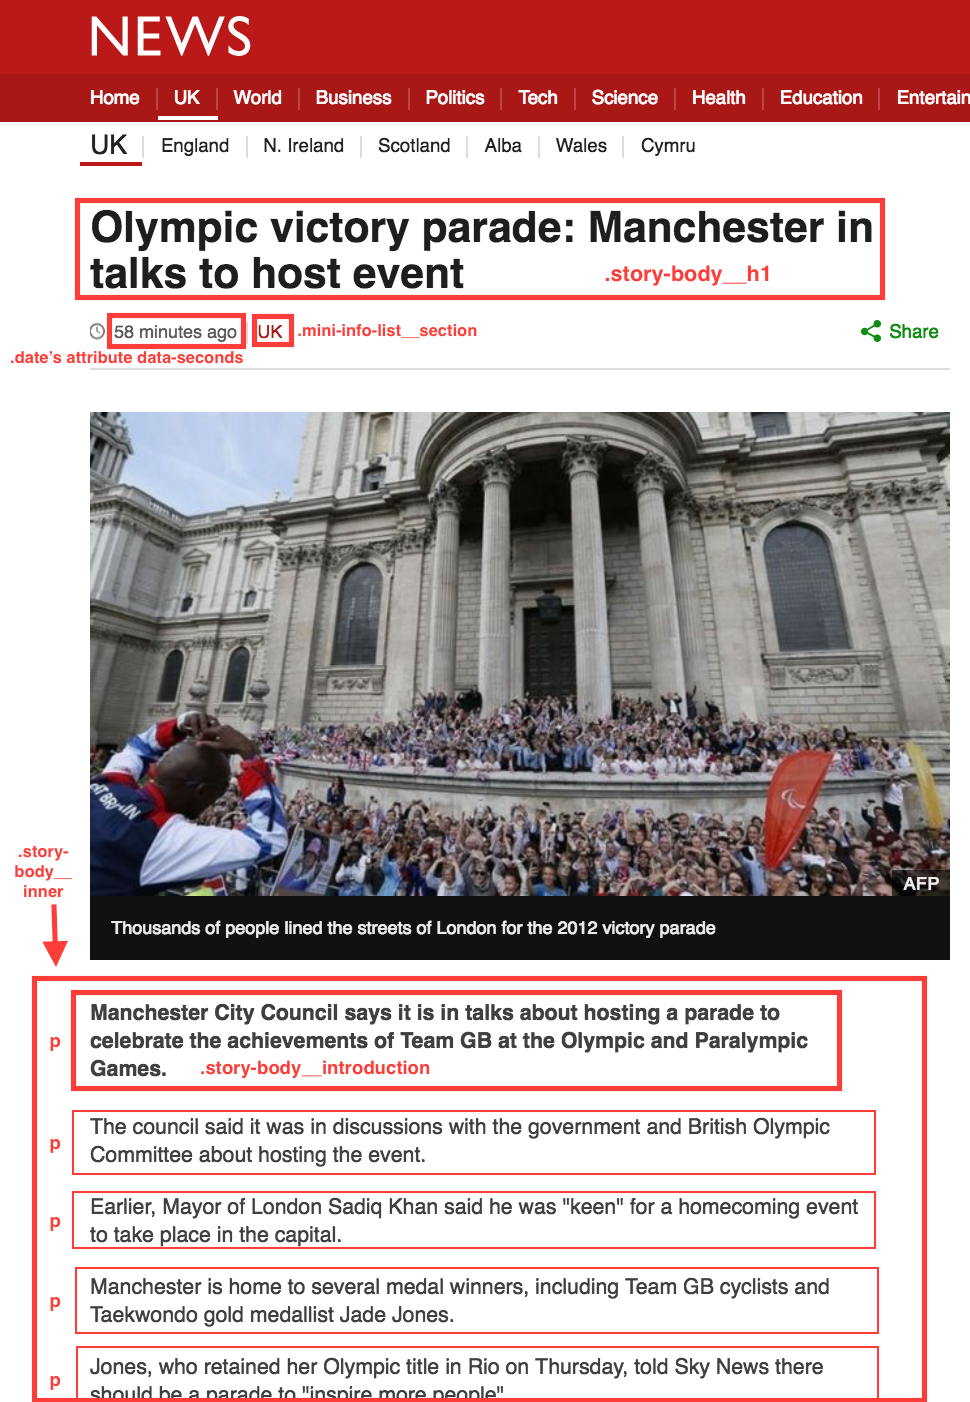
\includegraphics[scale=.9]{img/bbcArticle.png}
	\caption{Important BBC classes and attributes\label{fig:bbcArticle}}
\end{figure}

Sometimes on the BBC there are asides within articles that have the same tag that are not part of the article body; it is essential to remove them. They begin with \lstinline|<hr>| elements and can also end with them. By counting the number of \lstinline|<hr>|'s, the asides are removed. If the number modulus 2 is zero, it means that there is a single aside within the text which starts and ends with an \lstinline|<hr>|; paragraphs within those should not be added. If the number modulus 2 is one, there is either content below a single \lstinline|<hr>| that should be removed (it is probably a form or contact information for author), or there is at least one aside within the text followed by unnecessary content under the odd \lstinline|<hr>|. This method guarantees that only the article's text is processed. These checks conclude the extraction process. The paragraphs are stored as an array and other information as strings or numbers.

\subsection{Sentence Tokenizing}
Now that all article information is extracted, the paragraphs must be split into individual sentences. There are many difficulties associated with this because periods (``.'') not always mark ends of sentences.

Here, a library is used called ``natural'' to split the paragraphs into sentences. It provides many other natural language utility functions for Node.JS \cite{natural_node}. Given a paragraph, natural's sentence tokenizer returns an array of sentences. However, it is too aggressive on periods. This gets fixed by identifying two tokenizing errors: splitting on names and other likely cases. Splitting on names, such as ``Mr. Name'' is fixed by checking if the last word of the sentence is a title. If it is, then it is safe to concatenate this sentence and the next one. Potential titles are stored in a utilities file. The other case is if the sentence ends in a period but the next one begins with a lower-case letter (it could be an in-line URL), then it is also safe to concatenate the current and next sentences. 

Once the sentences are tokenized, sentences that are unfit to be part of a signature are filtered out. Since the signature is an extract, sentences that have only one pair of quotes are removed since it has an incomplete quote. Sentences that are within a quote are removed because they would not make sense taken out of context. For the same reason, sentences where a person is saying something are removed. After this operation, the remaining sentences represent the article's core content and the tokenization is finished.

\section{Text processing}
This module always follows the HTML parsing module. It gets given the result of the previous module as the argument. All implementation is found in \lstinline|textProcessing.js|.
\subsection{Word Tokenizing}
First, each sentence is tokenized into words as it is best for text processing. Using the sentences from the previous module, each one is tokenized into words and punctuation by the ``natural'' library's word tokenizer. There are no adjustments to make, unlike in sentence tokenization. The article is represented as an array of arrays of words/punctuation. 

There are additional processes that identify several classes of words. In each case, each sentence of the article is traversed to find a specific pattern. First comes detecting proper nouns. A proper noun is defined in this case as two or more words that begin with an upper case letter. Although this is a strong assumption, it is likely that if adjacent words are capitalized, they are related. The rationale for this is that the combined meaning of words is lost if they appear on their own, like in the case of ``New York City'' or ``David Cameron''. During sentence traversal, if a capitalized word is found, its index is flagged as the start of a potential proper noun. Once a word is found that is not capitalized, the difference between the start and end of the capitalized indexes is calculated. If it is bigger than one, it is considered a proper noun and it replaces all indexes that it was composed of. For example, the sentence \lstinline|["I", "live", "in", "New", "York", "City", "."]| becomes \lstinline|["I", "live", "in", "New York City", "."]|. A similar process happens to identify names (e.g. ``Mr. Cameron''), hyphenated words (e.g. twenty-four), URLs (e.g. yelp.com), and numbers (eg. 2,300,000). 

There were attempts to use a statistical measure to detect compound nouns, which are words that always appear together to represent a single concept, e.g. ``City of London''. If this type of word appeared more than two times, it could be considered a noun. However, BBC articles did not tend to say the same phrase more than once. 

Modularity is important for this component. Each function here takes and returns the same type of argument, which means that more steps can be added to the list of classes to detect if they take and return the same argument. The final result is each sentence adjusted to contain nouns that represent single entities. From now on, this is the only representation of the article that is used.

\subsection{Weighing words}
Another process begins to detect proper nouns. The motivation for this is to have another way of seeing if a word is a proper noun because proper nouns deserve a slightly higher importance during ranking. Each word of the article will appear as a key in an object, each beginning with a value of true. The article is traversed and each word is checked to see if it is upper-case at every occurrence. If an occurrence of lower-case is found, the word's value gets marked as false. A map of each word in the article with a flag marking it as always upper-case or not is created. This become the second representation of proper nouns.

Afterwards, the word frequencies of the article get calculated in two ways. The first way is a simple count of each unique word. The second way is the first step of calculating importance. The following formula is used: \[ \frac{number \ of \ occurrences \ of \ word}{number \ words \ in \ article} \times 100 \]. This formula represents the proportion each word takes up in the article. This is done to each word to get an initial value for its importance. This information is stored as key-value pairs, where the key is a word and the value is its importance. The words also go through a stemming process in a separate function using the Porter stemmer algorithm to get at the common roots of the words, as this will show which words are closely related. A library called porter-stemmer, found on node package manager, is used \cite{porter-stemmer}. Next, the average of the term frequencies gets calculated. This average will become crucial in the next steps.

A series of steps occur to adjust the importance of all words. First the article's headline is weighed. For each word of the headline that is not a stop-word, its importance gets increased by three times the average. This is because the headline likely contains important terms that the article is about. Similarly, the first sentence of the article gets weighed more, with each word receiving an additional importance of 1.5 times the average. On the BBC, this is the bolded sentence at the beginning of articles which already generally summarizes the contents. Additionally, if the name of the section appears in the text, it gets an additional importance of 0.5 because the user may simply be interested in reading news from that section. All words that are in the first half of the article get an additional importance of 0.75 times the average because sentences closer to the beginning of the article tend to be more relevant to the main topic. 

Next, stemmed words are weighed. For stems that have two or more words representing them, this process occurs. The importance weights of all words of the stem get added. The word with the highest weight gets chosen as the display word for that stem. That word gets assigned the sum of all weights. The other words get removed from the importance mapping. After the completion of this process, only one representation of each stem will remain. The motivation for this is that when it comes to choosing topic words, two words of the same stem are not chosen. The fact that the weight of the display word increases is good because it had other representations of it that were removed, therefore more occurrences. Surprisingly, testing this method in production does not affect the importance scores that much. The way articles are written on the BBC tends to have a lot of unique words, with the only stems being different word tenses (that do not count for topic words) and singular/plural nouns (which is best to have only one version of for topic words). The stems with more than one word are vastly outweighed by stems with only one word. However, it is still worthwhile to run this function because of the reasons stated above.

The final adjustment to word weights is weighing proper nouns. The proper nouns object which contains a mapping to either true or false is used here. The part-of-speech tagging functionality of the library called ``nlp-compromise'' is used. This library, which is found on node package manager, has many helper functions for processing natural language \cite{nlpcompromise}. It adds some additional checks to make sure no unimportant words are getting increased importance. Each unique word of the article gets checked to see if its a proper noun. If it is a name with a title (e.g. ``Mr. Cameron''), a date, value, or demonym, it is skipped. Otherwise, if it is a proper noun according to the mapping object, its importance gets increased by 2.5 times the average. This is because proper nouns are a much stronger concept than any regular noun and more strongly describe the contents of the article. This step concludes the word weighing. The words are then sorted in descending order of importance.

\subsection{Determining topic words}
Now that article words are weighed and sorted, the topic words of the article are determined. There are eight topic words extracted, but this number can change based on the parameter. 

The requirements state topic words must be any type of noun. Two part-of-speech tagging libraries are used to determine which words can be used: ``nlp-compromise'' and ``pos'', which is a library developed for Node.JS based on the Brill tagger \cite{pos-library}. There is more flexibility and fine-tuning by using two libraries because each can have its own interpretation of a word.

Hyphenated words are not used as topic words because they tend to be numbers. Names that have only titles and surnames in them are also skipped because they are ambiguous. Using ``nlp-compromise'', several bad parts-of-speech are defined: Date, Value, and Adjective. A single good tag Place is defined. Using ``pos'', there are no bad tags, only good tags: NN (regular noun), NNP (singular proper noun), NNPS (plural proper noun), and NNS (plural regular noun). The ``pos'' tags take precedence here, so if it is a noun, it moves onto the next check. If the word is not a noun, it checks if the word is a place. If it passes that, it goes to the next check of verifying that the word is not any of the bad tags. If it passes, the word gets added to the topic words. If those checks failed, it checks if the word is a proper noun; if it is, the word is added to the topic words. This process is done until the requested number of topic words is determined. 

This module has now finished and sends the result containing the topic words array, word weights, and all other intermediate steps.

\section{Signature Generation}
With the bulk of the work done by the previous module, signature generation is simplified. All implementation is done in \lstinline|signatureGeneration.js|.
\subsection{Ranking sentences}
To determine which sentences are important, each one gets an importance score calculated. Using the result from the previous module, the importance value of all composing words is summed up. 

To control the weights of the sentences, adjectives are not given any value because they only describe other words and are unimportant out of context. Additionally, to prevent the longest sentences from getting chosen, each sentence importance is divided by its length. Doing this evens out the field to do more fair comparisons based on word importance alone.

The top two sentences are chosen to be part of the signature. Three sentences may yield a more informative signature, but it can tend to be too long for a quick summary.
\subsection{Adjusting sentences}
There are a few steps taken to shorten the signature and make it more readable. Each step looks for specific patterns in the signature's sentences. 

The first is to remove past participles, such as ``have created'' and ``have gotten''. Each can be replaced with a simple past tense, ``created'' and ``got'', respectively. This shortens the signature by a few words. There is a mapping stored between past participles and past tenses for the most commonly used. 

Another method attempts to remove shorter clauses from the sentence that are separated by a comma, such as ``said reporters''. This is done by checking the position of commas in each sentence. If there is a comma in the first or last 20\% of the sentence, that part of the sentence is removed. It is often the case that those sections do not add anything meaningful except for minor clarification. Another check is for dashes. If there are two dashes, text between them is often for clarification as well. This can be removed from the signature as it is not essential for quick summaries.

There is a function that attempts to fix readability by replacing names with titles with the person's full name. By extracting the surname from the title and comparing it against the list of available proper nouns, if a surname match is found, the title is replaced by the entire name. The first match from the list is taken. If there are people with the same surname in the article, there is a risk that the wrong name may get chosen. Another check happens for sentences beginning with ``He'' or ``She''. If a sentence is found with that as the first word, the algorithm traverses backwards until a proper noun is found as the first word of a sentence.  This pattern was observed with BBC articles; sentences beginning with a person's name often have the next sentence beginning with ``he'' or ``she''. Once a match is found, the first word of the sentence is replaced by the proper noun.
\subsection{Sending the signature}
After modifying the sentences, they must be concatenated to look normal as they are still in array format. A string is built from the words and there are many rules as to when to add a space. Sometimes a space is not needed, like when there is a comma or period following the word. Special care is taken for quotation marks because a space is needed before an opening quote but no space before the closing one. Once this process completes, the response from this module is sent, which includes the signature and all intermediate steps.


\section{Retrieving New Updates}
This module is called independently of all other modules. It attempts to retrieve newer articles that are related to stories to show progression. Each update gets displayed on a story's timeline. All implementation is found in \lstinline|webCrawling.js|.
\subsection{Sending Request}
Each story has an attribute called \lstinline|modifiedTopicWords| which represents the tracked topics. It is a key-value object ordered by descending values. Initially, each word has the same weight but are still ordered by importance. These weights are important later on during user feedback. The user interface sends all these topic words in the request in order, the timestamp of the most recent article of the story, and the news category the article is from (i.e. news or sport).
\subsection{Getting search results}
The server performs a search on the BBC using the first two most relevant topic words. At first, three were used but sometimes there were no results found so the search criteria was too strict. Using two words was too general because articles that are unrelated were constantly found. There were two courses of action: using three topic words and accepting that there may not always be very specific updates or changing the algorithm for topic word detection. The latter was done to fix this problem, which led to the aforementioned steps of multiple ways of finding proper nouns and giving them higher weights. This improved topic word quality so only two topic words could now be used in the search since two words alone better portrayed the contents of the article.

A search URL is built using the category of the BBC and the topic words of the pattern \lstinline|http://www.bbc.co.uk/search?filter=CATEGORY&q=TOPIC+WORDS|. Performing a GET request gets the search results. The results are then extracted using the library ``cheerio'', like when parsing news articles. Three features of the articles are extracted: headline, timestamp, and URL.
\subsection{Choosing potential matches}
Each headline is compared against all topic words from the original request. If any of the topic words or their subsets appear in the headline, the article is flagged as a potential match. 

Timestamps were used to filter articles since ones older than the most recent in the story cannot be new developments. However, this step was dropped because the timestamps on the search results and the actual articles did not match.

All potential articles get parsed in the same way as any new article that is added by the user. Useful information is extracted and topic words and the signature are generated for each.
\subsection{Ranking potential matches}
Articles are first filtered on timestamps because older articles than the current newest can be automatically discarded. Articles that remain go through a ranking process. Each article is assigned points that represents how closely it is related to the story.

Relatedness is determined by a similarity score. The similarity score is calculated by comparing the topic word arrays of the story and new article for strength of overlap. For each exact match of topic words between the story and the article, the distance between the indexes is computed. For example, if the match appears in the first index of the story's topic words and in the third index of the article's topic words, the distance is two. The article's score is incremented by the following formula: \[ (w\,-\,k)\,+\,\frac{w}{distance\,+\,1}\,+\,j\]
where $w$ is the number of topic words generated by the system (eight in this case), $k$ is the index of the word in the story's array, and $j$ is the index of the word in the article's array. For every partial match, half of that calculated number is added to the article's score. This method takes into consideration that the words closer to the beginning of the topic words list are more important. Word matches are also rewarded if they are in the same index, which is done by a reciprocal function where the numerator is the number of topic words. Once all words are compared, that article's score is calculated. The process repeats for all potential articles.
\subsection{Choosing the next article}
The article with the highest score is selected as the next development for the story. In cases where there is only one potential article, it would get chosen as the development. However, it may not necessarily be related to the tracked story. The similarity score only works in relation to other potential articles. Consequently, a simple topic word overlap percentage is calculated. At least 25\% of the topic words must overlap to be considered a match. 

Once these checks conclude, the remaining article is sent to the user interface with its signature, timestamp, topic words, and headline. If no article was deemed relevant, a response is sent to the front-end saying that there were no new articles.

\section{Putting it all together}
\subsection{Creating an API}
Currently, all the above modules are individual entities. Some of these need to be combined into sequences of steps that can be easily called in a fixed order. The file \lstinline|storyevolutiontracker.js| contains several ``recipe'' functions that can be called to invoke these modules. There are two functions that the user interface requires: parsing an article to generate a signature and finding the next article for a story. The first one contains article extraction and parsing, text processing, and signature generation in order. The second only calls the retreving new articles module.
\subsection{Dealing with asynchronous code}
All these modules behave asynchronously, i.e. they do not block while they execute. To maintain an order of operations, each function had to have a callback as an argument, which would get called when the function finishes to begin the next step in the sequence. Because there are several steps for processing an article, this led to a lot of callback nesting. Each step had a callback which called another module that also contains a callback, and so on.

To fix this, the code was refactored to use JavaScript ES6 Promises which help for developing asynchronous code. Each Promise ``represents a single asynchronous operation that has not completed yet, but is expected in the future'' \cite{promises}. Code readability and modularity improved as new steps can be added to a sequence trivially. A single parameter gets passed through all functions so the flow of information is not impeded by the refactor. Refer to figure~\ref{fig:promises} for an example.

Each module's exported function (the one that can get called externally; normally the main function) returns a Promise. It is either resolved with a result or rejected with an error, so there is better error handling as a result. 
\begin{figure}[here]
\noindent\begin{minipage}{.45\textwidth}
\begin{lstlisting}[frame=tlrb]
one(arg, function() {
    two(arg, function() {
        three(arg, function() {
	        ...
        });
    });
});
\end{lstlisting}
\end{minipage}\hfill
\begin{minipage}{.45\textwidth}
\begin{lstlisting}[frame=tlrb]
one(arg)
    .then(two)
    .then(three)
    ....
\end{lstlisting}
\end{minipage}
\caption{On the left: before Promises.  On the right: after Promises.\label{fig:promises}}
\end{figure}

\section{User Interface}
An Android application is the user interface for the Story Evolution Tracker. It follows the design considerations from section \ref{design:ui}. A full user guide is in Appendix \ref{appendix:userGuide}.

\subsection{Retrieving Updates}
There are two ways the user can receive updates to their stories. One way is to pull the screen to refresh each story, and another way is background updates, which are set to every hour. The user would be able to change this in the settings. A separate request is made to the server for each tracked story to get new articles. If there is something found, the story's most recent timestamp and signature get updated and this change is visible on the screen.

\subsection{User Feedback}
If an article is selected that does not match what the user wants to read about, the user can down-vote it. On the other hand, if they know this is exactly what they wish to read about, the user can up-vote it.

Each update comes with its own topic words. In addition, each story has an object called \lstinline|modifiedTopicWords| which maps topic word and strength. When a user down-votes an article, each topic word of the article will decrease the strength of those words in \lstinline|modifiedTopicWords|. Up-voting increases the strength of those words. 

A number is calculated for each index which represents how much is to be added or subtracted which is inversely proportional to the number of topic words in the story and the word's index in the list. For example, if a user down-votes an article and there are eight topic words, the first word would have its corresponding entry's strength in \lstinline|modifiedTopicWords| decreased by eight. Up-voting would increase the word's strength by eight. This approach was chosen because the words closer to the beginning of the list are more relevant to the article and words towards the end are more loosely related.

\subsection{Storing data}
There are several options for storing user data, such as using a database on the server or using the device's internal storage. An advantage to using the server is that the user would be able to log-in from multiple devices to view their tracked stories, but authentication would need to be put in place. Using device internal storage is much simpler to implement, but if the data is lost, so are the tracked stories. For simplicity, the application uses internal storage.

This leads into deciding the format of user data. Since Android runs on Java, options include Java objects or JSON. Java objects are simple to implement due to the object-oriented nature, but there is some overhead when converting them to a format suitable for storage. JSON is slightly tougher to use in Java because of object wrappers, but since the server gives responses in a JSON format, it is advantageous to use JSON. All user data including stories and timelines are stored in JSON as a result. The schema for these can be found in Appendix \ref{appendix:userData}.

\chapter{Testing and Evaluation}
\section{Overview}
This chapter will go into the testing and evaluation procedures for the Story Evolution Tracker. The goal is to see if the system meets expectations in terms of specifications, performance, and many other qualities.
\section{Testing}
The system was tested with the use of a simple web application that was built for this purpose. Additionally, a Google Chrome extension PostMan was used to test sending GET and POST requests and receiving responses \cite{postman}.
\subsection{HTML Extraction and Parsing Quality}
The system can be given any text to process. There are many error checks in place throughout the extracting and parsing process to make sure that the system does not crash. For cases when the given text is not a URL, the system terminates and returns the message ``Neither a file nor http url''. However, it is the client-side's responsibility to make sure that the URL that is passed is a real website because \lstinline|http://hello| is still considered a correctly formatted URL. Other checks include whether the URL is a supported source; if not, the system returns a message saying ``Not a BBC News or BBC Sport article''. When HTML parsing occurs, all necessary parts of the article are extracted. If any parts are missing, an error is returned with ``Article is not suitable for tracking''. Resiliency to various inputs is an important aspect of this module. The quality of the extracted text is high: string fields are trimmed of excess spaces and paragraphs are returned in order.
\subsection{Topic Word and Ranking Quality}
The topic word quality depends on the word rankings. There are always at least five words chosen, unless an articles has very few words. Topic word quality is high, but it is not perfect. Although multiple measures are in place to to ensure that all topic words are nouns, many words are ambiguous. For example, the word ``supports'' can be a noun or a verb, but it is impossible to tell with the current tagging mechanisms. On the other hand, the emphasis on proper nouns is proving to be useful with very specific topics appearing often in the topic words arrays.

Unfortunatly, there are cases when words appear that are subsets of others. This is a waste of a topic word slot since the concept is represented already. There is also a bug in the system where some importance value gets set as a key in the object where the mappings are kept. This however does not affect anything because it is filtered out by the part-of-speech tagging libraries.
\subsection{Signature Quality}
Two sentences are always selected for the signature, unless there are fewer sentences in the article. The extracted sentences always appear in chronological order. Signatures always contain some of the topic words because those words were weighed the highest and gave those sentences the highest importance values. Sentences often make sense out of context, but potentially not always. Due to the nature of the extract, sentences can be taken from anywhere in the article. There is sometimes a lack of cohesion between the two sentences because they were not adjacent in the article. Other times, a person may still be referred to by their title and surname, even if an effort was made to replace titles by their full names. Additionally, sometimes sentences begin with ``He'' or ``She'', which also does not make sense out of context. Even though there is a function that attempts to fix this, there is potential for the wrong name to be chosen to replace the pronoun.

Signatures often capture the main topic of the article because of how heavily weighed the top of the article is. However, there are sometimes cases where the sentences do not explain the article very well. For example, this signature ``Choudary was convicted alongside confidant Mohammed Mizanur Rahman. Choudary and Rahman will be sentenced at the Old Bailey on 6 September.'' does not serve well as a first summary since there is no background information. However, it may fit as an update to a story where the user already knows the background.

There is also a minor bug with punctuation that is improperly spaced because not all cases can be accounted for. 
\subsection{Update Quality}
Articles that are chosen are normally quite closely related to the story by a few topic words. If anything, the stories tend to be a bit more general. After testing the automatic updates for about a week, there were very successful and interesting results.

Tracking a story with the first few topic words as ``gold'', ``gb'', and ``rio olympics 2016'' was finding all articles about Team GB in the Olympics when it won a gold medal. Between August 12 and August 17, fourteen stories were found automatically about different events where a gold medal was won. Including which section the articles came from greatly improved finding new ones.

A story tracking an oil rig in Western Isles, Scotland managed to get very specific articles. The first few topic words were ``western isles'', ``rig'', and ``transocean winner''. It was surprising to get an update after not having received any for a few days. The article that was extracted was a clear continuation of the story.

However, one story which was tracking the topic words ``britain'', ``usa'', and ``gymnastics'' started giving very general articles, such as ones about swimming and cycling. This is where the user feedback really allowed to fine tune which articles the algorithm was finding.
\subsection{User Interface}
The user interface tries to prevent a lot of actions that would crash the system. All text input fields have client-side checks to ensure that no poorly-formatted data gets sent to the server. Other testing techniques included going between the screens to make sure the data is still there. This would test if data was stored correctly. 

Changes had to be made in terms of using user data throughout the application. At first, it was sent through the screens as an extra for an intent, or in other words, as a parameter. However, this led to data inconsistencies, so this was fixed by every time any operation happened on the data, it would get saved right away. Other screens would load it, so there were no more inconsistencies.
\section{Evaluation}
\subsection{HTML Extraction and Parsing Module}
This module is responsible for which news sources are supported. Adding new sources is not very difficult so there should be some ones added. The benefit of having multiple sources is different points of view as well as a variety of information for news events.

A smaller improvement that could be made is removing the dependency on the ``natural'' tokenizing library. A dedicated parser can be written that can handle punctuation more delicately as to not require the concatenation of sentences later on.
\subsection{Text Processing Module}
This module can be improved by better named entity recognition. Currently words like ``Theresa May'' and ``PM Theresa May'' are considered distinct. The beginnings of sentences should also be taken into consideration when determining proper nouns. If the first word is not a stop word and it is followed by a proper noun, it would get included as part of the proper noun, e.g. ``Brilliant Simone Biles is a gynmast'' would detect ``Brilliant Simone Biles'' as a proper noun. Other proper nouns still cannot be detected such as ``Rio de Janeiro'' because the connecting word is lower-case. This is more significant if the connecting word is a stop-word.

Different importance values can be assigned to sections of the article when weighing words. They are currently set based on some intuition and guessing-and-checking.
\subsection{Signature Generation Module}
A lot of techniques were attempted to try to shorten the signature. When the signature was set to three sentences, shortening techniques made sense to do. First, there was a simple black-list of words that were removed from the signature, which included ``the'', ``an'', and ''a''. It performed well to shorten the signature. However, when the signature was reduced to two sentences, removing these words did not add much value and only decreased readability. A similar thing was attempted with possessive words but also did not perform well. 

Another attempt was to remove adjectives from sentences. Some adjectives that simply describe nouns can be removed without removing the meaning of the sentence. But due to the imprecision of the part-of-speech taggers, too many words would be removed, even after manually trying to find adjective, noun patterns that would be safe. The meaning of the sentence began to suffer. 

A final attempt was to remove some sentence clauses entirely. For instance, in ``He went outside on Friday'', the clause ``on Friday'' can be removed to summarize even further. Using the part-of-speech tagging libraries, good results were observed when looking at which clauses were extracted from a sentence. However, the difficulty came when determining which clauses can be safely removed. Removing all clauses would sometimes take out all useful information. This was a problem that was very difficult to solve, so clauses remain in the signature. The code remains for potential future work.
\subsection{Retrieving new Updates Module}
Currently only one page of results is taken from the BBC. Although this is normally fine since results are ranked in order of relevance and date, for very active stories with many articles, results may be on a second page. As stated during the design, if the system is to expand, the searching may need to change.

Additionally, the BBC tends to update its articles rather than posting new ones for active topics. This means that the timestamp changes yet very little may have been added to the article. This algorithm would consider this to be a new article and generate a signature for it, which would end up being identical to the previous article since it still finds the most relevant sentences. One way of fixing this would be to send the whole story timeline in the request. If an article that already appears in the timeline is chosen, previously-used sentences could be flagged in the article to not use in the signature again. Therefore, a different signature could be generated.
\subsection{User Interface}
Storing data in a JSON format makes it very simple to manipulate, but with a lot more overhead in Java. A lot of lines of code are written to write and save some data for a small part of the user. The change has to propagate through the entire user object. The files with the application logic could benefit from a reorganization but this is minor. Overall, the application performs well with no known situations where it would crash.
\subsection{General and Performance Evaluation}
Overall, the project meets the specification. The design considerations were followed and were amended when needed. As performance goes, it may not be performing at its best. One instance is where there are many cases of words to detect in the sentences, such as proper nouns and hyphenated words. For each case, each sentence has to be traversed again, which makes a runtime of $O(m \cdot n)$, where $m$ is the number of sentences and $n$ is the length of the longest sentence.

Although there are many loops in that case, the performance does not compare to retrieving new articles, which is much slower. Updating each story takes a couple of seconds. This is because a GET request needs to be made for the search results and then there is another GET request performed for each potential article. Operations over the network are by far the slowest step. For this reason, background updates were implemented in the application. The user would not notice the slow performance if they are not doing manual updates themselves, which are still possible if the screen is pulled to refresh. The frequency of the background updates can be configured to the user's liking.

All things considered, the project meets its aims and additional technical information can be found in Appendix \ref{appendix:serverInfo}.

\chapter{Conclusions and Future Work}
\section{Conclusions}
The Story Evolution Tracker is the news application that was missing yet everyone needed. Many news applications attempt to give personalized news, but not on this level. Users specify a link to a news story they want to know more about. The system summarizes it and displays it as a tracked story. They get notified of any new developments and see the story's progression on a timeline, each one with a short summary. A set of topic words quickly identify which topics are being tracked. 

Users nowadays want a quick, personalized, and mobile news experience. The Story Evolution Tracker does this by summarizing articles, retrieving new articles that relate to their tracked topics, and proving an Android application that display all the information. Based on the statistics presented during the project motivation, the Story Evolution Tracker will be successful, should it be released to the public.
 
\section{Future Work}
There are many possible extensions to this project that could be done with more time. An obvious extension is support for more news sources to get a variety of information. 

Another idea is to have generic article suggestions for users. This would involve learning and tracking the user's interests. This can already be deduced in some ways because of which articles the user submits to track and which articles they up-vote or down-vote during feedback. The topic words that are determined for these stories and articles can be the interests that the user has tracked. Long-term and short-term interests can be used to more finely learn about the user's preferred topics. Similar methods to finding new articles for existing stories can be used to find generic articles based on the user's interests. This system can be added to the Story Evolution Tracker because a lot of the code infrastructure can be reused.

Finally, cloud support and authentication can be added to store user data. This would require some changes in the back-end but mostly in the front-end with regards to how data is stored in the application. This would allow users to have the application on multiple devices and not worry about any data getting deleted if their device is lost or broken. It would also be stored securely due to authentication. 

Relating to cloud support, there could be common data stored between all users that can help with either signature generation, proper noun identification, or article suggestions. Currently, all devices perform all tasks independently of one another, but if they were to communicate with a single entity, the aforementioned areas of the process could be improved. Some sort of data structure representing all proper nouns that are ever detected could be used to make proper noun identification quicker during text processing. It would also be more precise since many devices would strengthen the existence of each proper noun. Additionally, an ontology of words could be used across all devices to improve identification of similar words, which could improve word weighing and therefore signature generation. With regards to suggestions, many user models could be learned from to more accurately predict which articles users may like.

Simple improvements to the application would also be beneficial. Validity checks so the user cannot track the same article twice would improve the user experience because they would not mix up multiple stories. Additionally, some stories may have more updates than others. It would be nice to include functionality for setting background update frequency per story.

There are many more directions the Story Evolution Tracker could go. With more time, many more features could be implemented that would further improve the user experience.

% ------------------ REFERENCES ----------------------- %
\bibliographystyle{plain}
\bibliography{literature}

%---------------------- APPENDIX -----------------------%
\appendix
\chapter{User Guide}\label{appendix:userGuide}
\section{Main Screen}
\begin{wrapfigure}{l}{0.5\textwidth}
	\vspace{-1cm}
	\begin{center}
		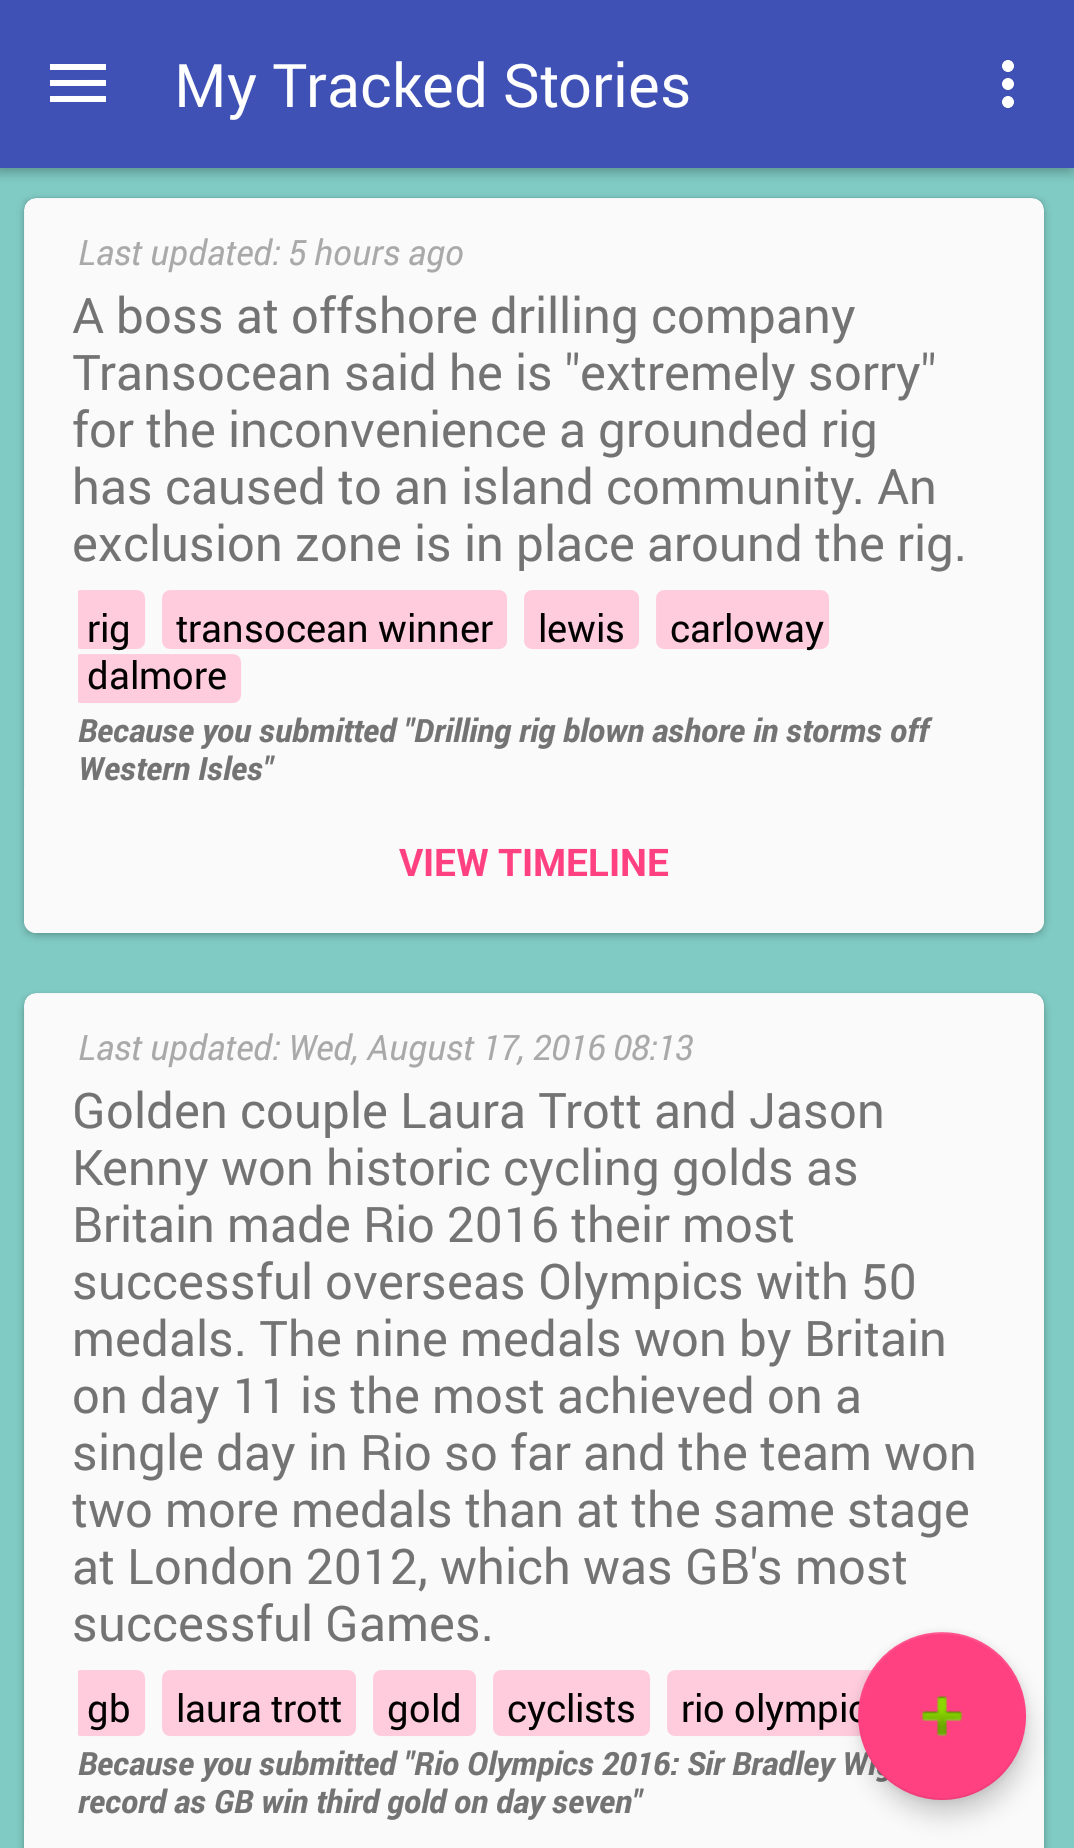
\includegraphics[width=0.5\textwidth]{img/mainScreen.png}
	\end{center}
	\caption{Main Screen}
	\vspace{-4cm}
\end{wrapfigure}
This is the main screen of the application. Each story is viewed as an individual card on the screen. If there are no tracked stories, it will say so on the screen instead of the cards. Clicking ``View Timeline'' will show the progression of the story.

Each story can be identified by two things: the topic words, which have the pink background, and the headline of the article that was originally submitted for this story.

The signature displayed is of the last development to have occurred. The timestamp is displayed relative to the current time and will show a full timestamp if the last development was more than 12 hours ago.

Stories can be refreshed manually by pulling the view to refresh. Otherwise, stories can update in the background and users can receive notifications if there is something new.

New stories are added by pressing the round plus button on the bottom-right of the screen.
\newpage
\section{Timeline View}
\begin{wrapfigure}{R}{0.5\textwidth}
	\vspace{-1cm}
	\begin{center}
		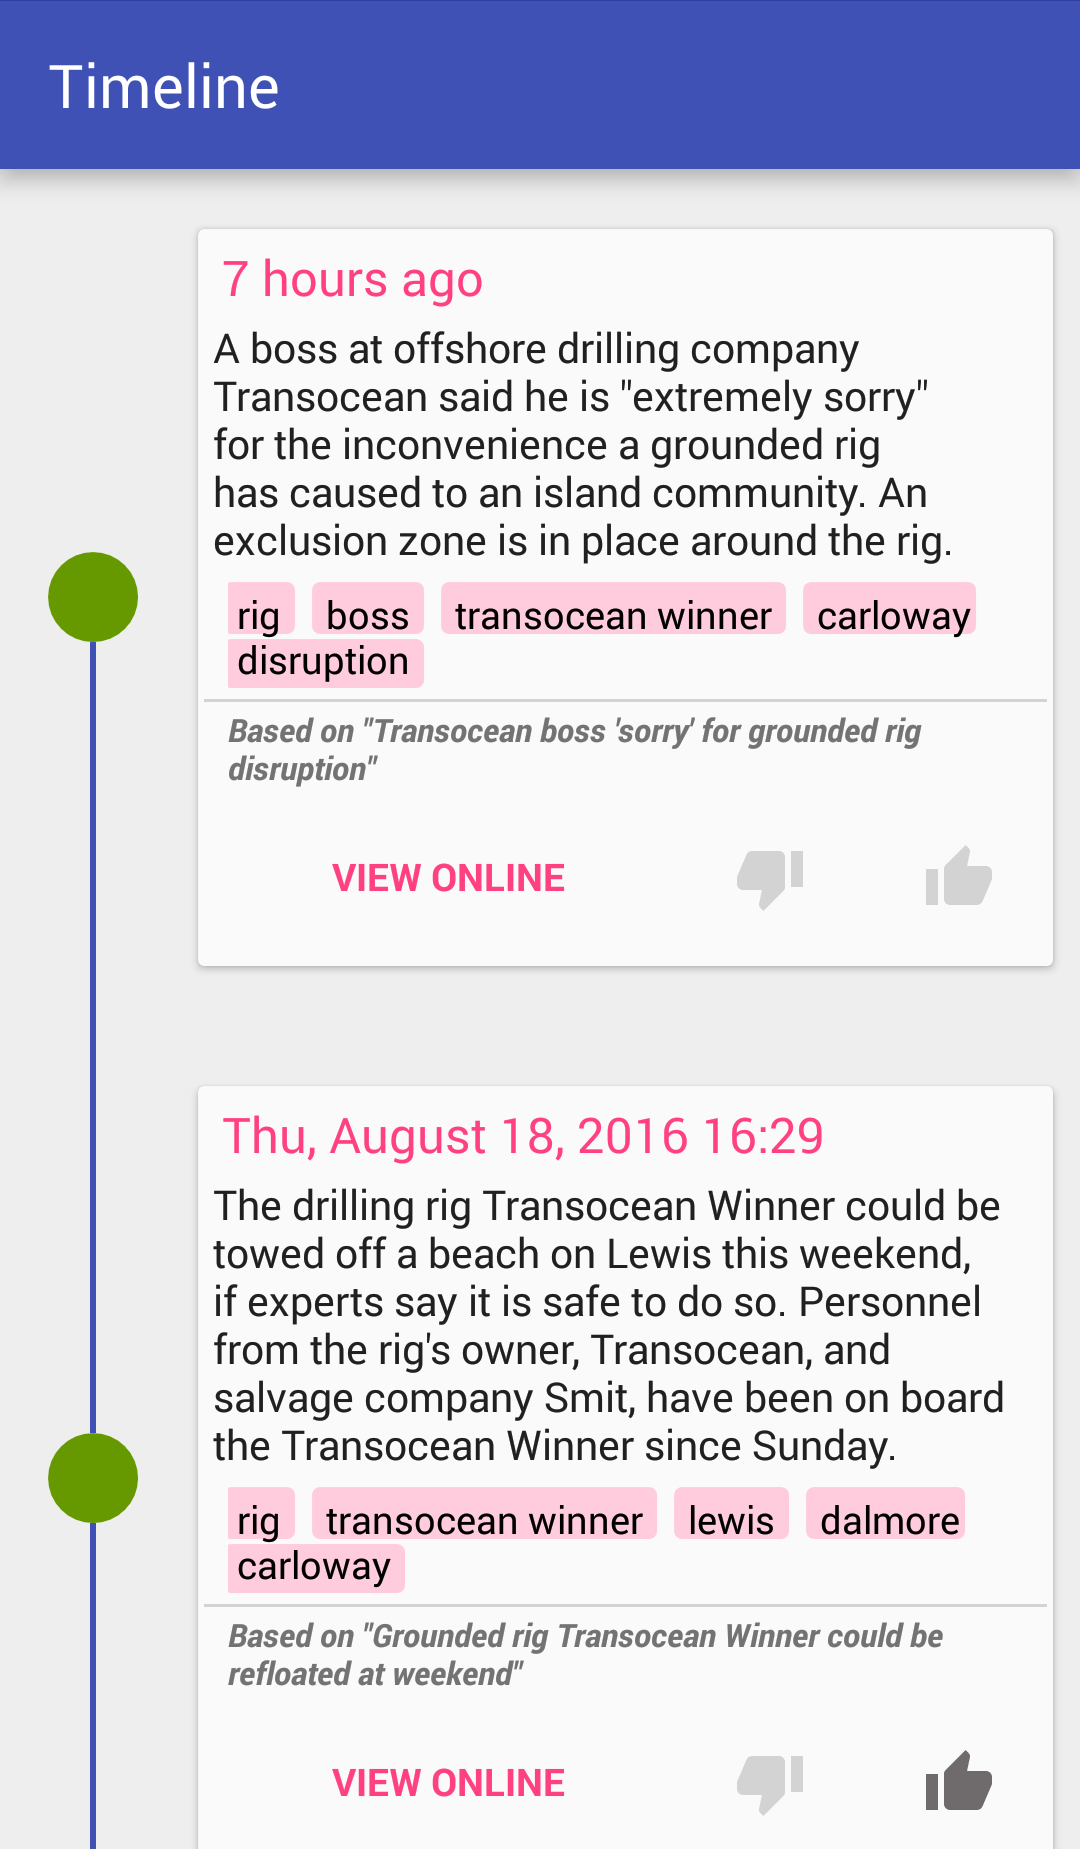
\includegraphics[width=0.5\textwidth]{img/timeline.png}
	\end{center}
	\caption{Timeline View}
	\vspace{-7.5cm}
\end{wrapfigure}
After clicking on a story in the main screen, this view is shown. Each entry in the timeline is a development that was found for the story. The most recent development is on top of the timeline.

Every entry displays a timestamp, a signature, topic words, and the headline of the article that it represents. The user has the option to view the article online to see the whole text.

Additionally, the thumbs-up button allows the user to give positive feedback on the article. Positive feedback strengthens the story to be about that article's topic words. The thumbs down button decreases the value of the topic words for that article. Only one of these buttons can be activated at a time if the user provides feedback.
\newpage
\section{Adding New Stories}
\begin{wrapfigure}{L}{0.5\textwidth}
	\vspace{-1cm}
	\begin{center}
		
\includegraphics[width=0.5\textwidth]{img/addNewStory.png}
	\end{center}
	\caption{Adding New Story}
	\vspace{-3cm}
\end{wrapfigure}
This is the screen where the user enters the URL of the news article to track. There are checks in place so the user enters only valid URLs. 

To make it simple to enter URLs, the user can press the ``Paste from Clipboard'' button which will populate the text field with the contents of the device's clipboard instead of having to press-and-hold the text field to paste.

Also, to make it even easier, the following is implemented. If the user is using the BBC News application, there is a share option on the screen. If they choose ``Copy to Clipboard'' from the list of options, the article headline and URL get put into the device's clipboard. If the user pastes this into the text field, both headline and URL, it will still work. Regular expressions extract the URL from the input. 

Once the user hits ``Begin Tracking'', a confirmation screen comes up with the article's details. Here the user can confirm or cancel. If they confirm, a story is created and is shown on their main stories screen.
\newpage
\section{Managing Stories}
\begin{wrapfigure}{R}{0.5\textwidth}
	\vspace{-1cm}
	\begin{center}
		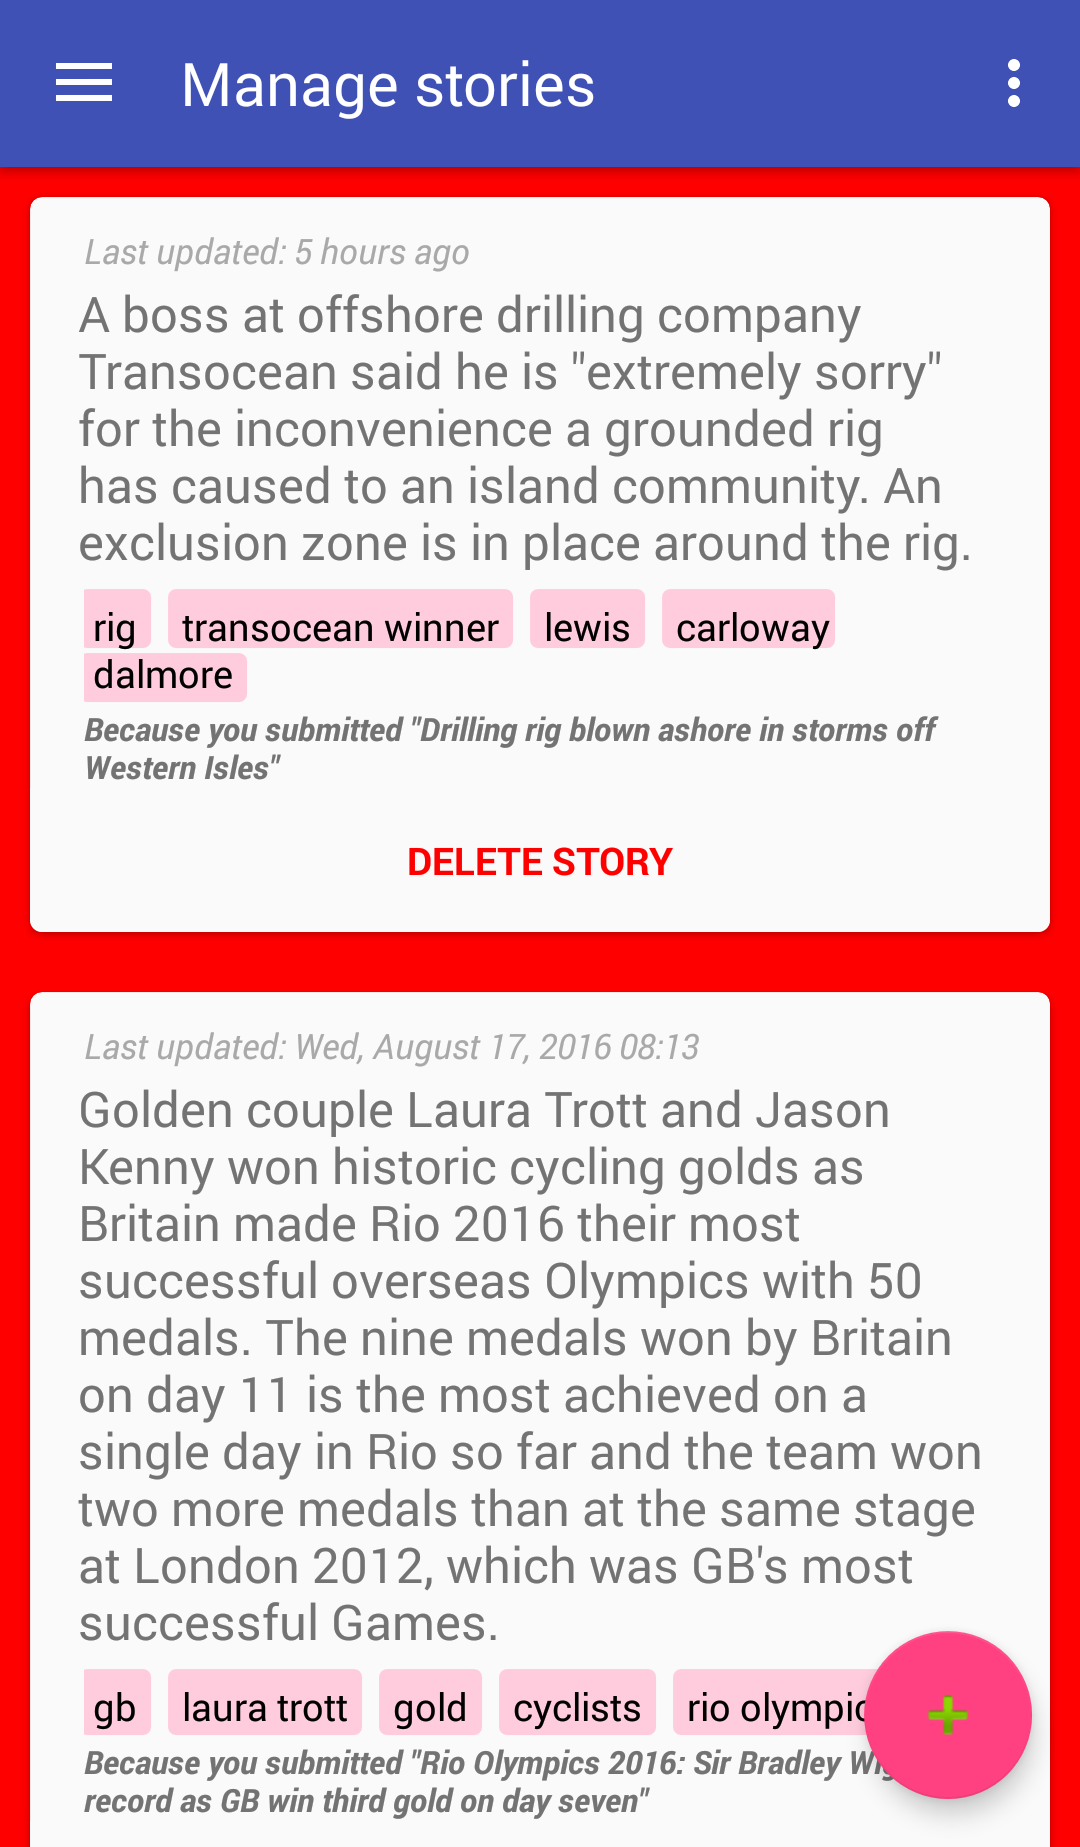
\includegraphics[width=0.5\textwidth]{img/manageStories.png}
	\end{center}
	\caption{Managing Stories}
	\vspace{-11.5cm}
\end{wrapfigure}
The user can manage which stories are being tracked. When the user presses the ``Delete Story'' button, a confirmation dialog opens. When the user confirms the deletion, that story is removed from their profile. 

If the user wishes to delete all their stories, there is an option to do so in the Settings.
\newpage
\section{Settings}
\begin{wrapfigure}{L}{0.5\textwidth}
	\vspace{-1cm}
	\begin{center}
		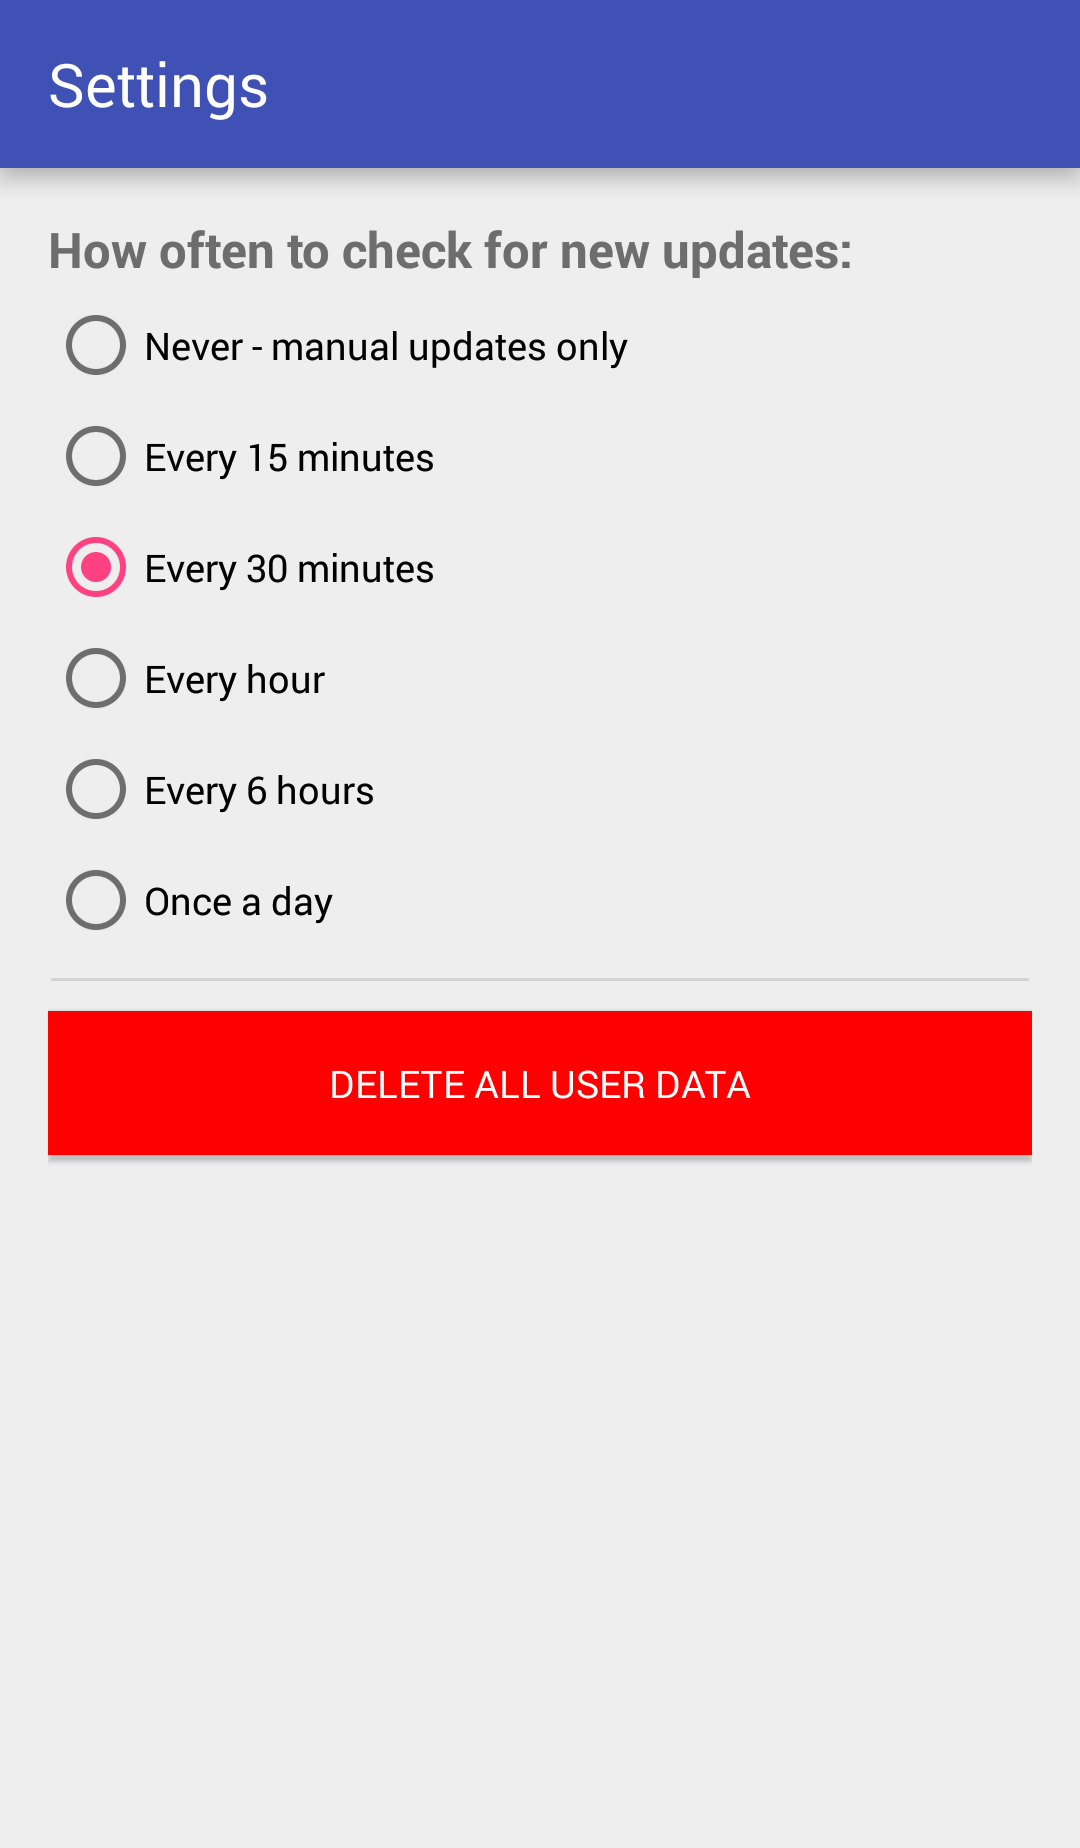
\includegraphics[width=0.5\textwidth]{img/settingsScreen.png}
	\end{center}
	\caption{Settings Screen}
	\vspace{-2.5cm}
\end{wrapfigure}
This is the settings screen which can be accessed from all main screens. The user can set the frequency of background updates, which will set how often the application will automatically get new developments. Pressing an option saves it right away. 

The user can also delete all their data with the red ``Delete all user data'' button. A confirmation screen will come up, and upon confirming, the application will go back to the original new user welcome screen. 

\chapter{Server Information}\label{appendix:serverInfo}
\section{Technical Details}
\renewcommand{\arraystretch}{1.5}
\begin{tabular}{>{\bfseries}l l}
IP Address and port of Application & http://139.59.167.170:3000/ \\
Host & DigitalOcean \\
Operating System & Ubuntu 16.04.1 \\
Node.JS Versions Supported & Node v4.5.0 and above
\end{tabular}

\section{Request Schemas}
\subsection{Signature generation}
\begin{tabular}{>{\bfseries}l l}
Route Address & \lstinline|http://139.59.167.170:3000/process_article| \\
HTTP Method & \lstinline|POST| \\
Parameters & \parbox[t]{10cm}{\lstinline|url_field| (the URL to process, encoded), \\ \lstinline|prod| (true for user interfaces, false for development)} 
\end{tabular}
\subsection{Retrieving new articles}
\begin{tabular}{>{\bfseries}l l}
	Route Address & \lstinline|http://139.59.167.170:3000/get_next_article| \\
	HTTP Method & \lstinline|POST| \\
	Parameters & \parbox[t]{12cm}{\lstinline|timestamp| (of most recent article in story), \\ \lstinline|category| (which section of the BBC, news or sport), \\ \lstinline|words| (each topic word of story sent with this, eg \lstinline|words=london&words=uk&...|)} 
\end{tabular}

\section{Response Schemas}
\subsection{Signature generation}
\begin{lstlisting}
    {
        "success": (true or false; if false, remainder of response is an error message),
        "link": (string: the URL from the user),
        "date": (number: timestamp of the article in seconds),
        "section": (string: specific news category),
        "headline": (string: headline of article),
        "category": (string: which part of the BBC, news or sport),
        "topicWords": (array: topic words representing article),
        "topicWordsFreq": (object: same topic words but set up as key-value pairs, where values are all 1; this is for user-feedback in UI),
        "signature": (string: signature of article)
    }
\end{lstlisting}
\subsection{Retrieving new articles}
\begin{lstlisting}
    {
        "found": (true or false; if false, remainder of response is message saying no article found),
        "link": (string: URL to new article),
        "headline": (string: headline of new article),
        "date": (number: timestamp of article in seconds),
        "section": (string: specific news category),
        "topicWords": (array: topic words of new article),
        "signature": (string: signature of new article)
    }
\end{lstlisting}

\chapter{User Data Storage in Application}\label{appendix:userData}
\section{User Schema}
\begin{lstlisting}
    {
        "username": (string: the name the user specifies),
        "updateFreq": (string: represents how often the tracked stories update in the background)
        "topics:" (array: each index is a tracked story; see next section for schema of each index)
    }
\end{lstlisting}
\section{Story Schema}
\begin{lstlisting}
    {
        "originalTopicWords": (array: words from the originally submitted article),
        "originalHeadline": (string: headline of originally submitted article),
        "lastTimeStamp": (long: time in seconds of most recent article),
        "lastSignature": (string: signature of most recent article),
        "lastUpdated": (long: system time when the story was updated),
        "category": (section of BBC original article is from, news or sport),
        "id": (random unique id assigned so notifications are optimized)
        "modifiedTopicWords": (object: tracks strength of topic words for user feedback),
        "timeline": (array: each development of the story; see the next section for schema of each index)
    }
\end{lstlisting}
\section{Timeline Entry Schema}
\begin{lstlisting}
    {
        "link": (string: link to article),
        "date": (long: timestamp of article in seconds),
        "section": (string: specific news category of article),
        "headline": (string: headline of current article),
        "category:" (string: section of BBC),
        "topicWords": (array: words for current article),
        "signature": (string: of current article),
        "thumbsUp": (boolean: true if user pressed, false if not; only one of these is true at one time),
        "thumbsDown": (boolean: true if user pressed, false if not; only one of these is true at one time)
    }
\end{lstlisting}
\chapter{Source Code}
\newcommand{\includecode}[1]{\lstinputlisting[basicstyle=\footnotesize\ttfamily]{#1}}
\section{Server Code}
\subsection{storyevolutiontracker.js}
\includecode{/Users/violet/Development/StoryEvolutionTracker/server/storyevolutiontracker.js}
\subsection{htmlParser.js}
\includecode{/Users/violet/Development/StoryEvolutionTracker/server/htmlParser.js}
\subsection{parsers.js}
\includecode{/Users/violet/Development/StoryEvolutionTracker/server/parsers.js}
\subsection{textProcessing.js}
\includecode{/Users/violet/Development/StoryEvolutionTracker/server/textProcessing.js}
\subsection{signatureGeneration.js}
\includecode{/Users/violet/Development/StoryEvolutionTracker/server/signatureGeneration.js}
\subsection{webCrawling.js}
\includecode{/Users/violet/Development/StoryEvolutionTracker/server/webCrawling.js}
\subsection{util.js}
\includecode{/Users/violet/Development/StoryEvolutionTracker/server/util.js}
\subsection{routes/index.js}
\includecode{/Users/violet/Development/StoryEvolutionTracker/server/routes/index.js}

\subsection{app.js}
\includecode{/Users/violet/Development/StoryEvolutionTracker/server/app.js}
\subsection{www (Start script for server)}
\includecode{/Users/violet/Development/StoryEvolutionTracker/server/scripts/www}
\section{Development Web App Code}
\subsection{public/index.html}
\includecode{/Users/violet/Development/StoryEvolutionTracker/server/public/index.html}
\subsection{routes/signatures.html}
\includecode{/Users/violet/Development/StoryEvolutionTracker/server/routes/signatures.html}
\subsection{routes/crawler.html}
\includecode{/Users/violet/Development/StoryEvolutionTracker/server/routes/crawler.html}
\subsection{public/stylesheets/style.css}
\includecode{/Users/violet/Development/StoryEvolutionTracker/server/public/stylesheets/style.css}
\section{Android Application Code}
\subsection{MainActivity.java (com.storyevolutiontracker)}
\includecode{/Users/violet/Development/StoryEvolutionTracker/Android/StoryEvolutionTracker/app/src/main/java/com/storyevolutiontracker/MainActivity.java}
\subsection{GetUserName.java (com.storyevolutiontracker)}
\includecode{/Users/violet/Development/StoryEvolutionTracker/Android/StoryEvolutionTracker/app/src/main/java/com/storyevolutiontracker/GetUserName.java}
\subsection{NewsHomeScreen.java (com.storyevolutiontracker)}
\includecode{/Users/violet/Development/StoryEvolutionTracker/Android/StoryEvolutionTracker/app/src/main/java/com/storyevolutiontracker/NewsHomeScreen.java}
\subsection{AddNewStory.java (com.storyevolutiontracker)}
\includecode{/Users/violet/Development/StoryEvolutionTracker/Android/StoryEvolutionTracker/app/src/main/java/com/storyevolutiontracker/AddNewStory.java}
\subsection{ConfirmArticle.java (com.storyevolutiontracker)}
\includecode{/Users/violet/Development/StoryEvolutionTracker/Android/StoryEvolutionTracker/app/src/main/java/com/storyevolutiontracker/AddNewStory.java}
\subsection{ViewTimeline.java (com.storyevolutiontracker)}
\includecode{/Users/violet/Development/StoryEvolutionTracker/Android/StoryEvolutionTracker/app/src/main/java/com/storyevolutiontracker/ViewTimeline.java}
\subsection{StoriesViewAdapter.java (com.storyevolutiontracker)}
\includecode{/Users/violet/Development/StoryEvolutionTracker/Android/StoryEvolutionTracker/app/src/main/java/com/storyevolutiontracker/ViewTimeline.java}
\subsection{TimelineViewAdapter.java (com.storyevolutiontracker)}
\includecode{/Users/violet/Development/StoryEvolutionTracker/Android/StoryEvolutionTracker/app/src/main/java/com/storyevolutiontracker/ViewTimeline.java}
\subsection{ManageStoriesAdapter.java (com.storyevolutiontracker)}
\includecode{/Users/violet/Development/StoryEvolutionTracker/Android/StoryEvolutionTracker/app/src/main/java/com/storyevolutiontracker/ManageStoriesAdapter.java}
\subsection{SettingsScreen.java (com.storyevolutiontracker)}
\includecode{/Users/violet/Development/StoryEvolutionTracker/Android/StoryEvolutionTracker/app/src/main/java/com/storyevolutiontracker/SettingsScreen.java}
\subsection{StoriesViewFragment.java (com.storyevolutiontracker.fragments)}
\includecode{/Users/violet/Development/StoryEvolutionTracker/Android/StoryEvolutionTracker/app/src/main/java/com/storyevolutiontracker/fragments/StoriesViewFragment.java}
\subsection{ManageStoriesFragment.java (com.storyevolutiontracker.fragments)}
\includecode{/Users/violet/Development/StoryEvolutionTracker/Android/StoryEvolutionTracker/app/src/main/java/com/storyevolutiontracker/fragments/ManageStoriesFragment.java}
\subsection{UserProfileFragment.java (com.storyevolutiontracker.fragments)}
\includecode{/Users/violet/Development/StoryEvolutionTracker/Android/StoryEvolutionTracker/app/src/main/java/com/storyevolutiontracker/fragments/UserProfileFragment.java}
\subsection{HelpFragment.java (com.storyevolutiontracker.fragments)}
\includecode{/Users/violet/Development/StoryEvolutionTracker/Android/StoryEvolutionTracker/app/src/main/java/com/storyevolutiontracker/fragments/HelpFragment.java}
\subsection{AboutFragment.java (com.storyevolutiontracker.fragments)}
\includecode{/Users/violet/Development/StoryEvolutionTracker/Android/StoryEvolutionTracker/app/src/main/java/com/storyevolutiontracker/fragments/HelpFragment.java}
\subsection{ValuesAndUtil.java (com.storyevolutiontracker.util)}
\includecode{/Users/violet/Development/StoryEvolutionTracker/Android/StoryEvolutionTracker/app/src/main/java/com/storyevolutiontracker/util/ValuesAndUtil.java}
\subsection{UpdateNewsReceiver.java (com.storyevolutiontracker.util)}
\includecode{/Users/violet/Development/StoryEvolutionTracker/Android/StoryEvolutionTracker/app/src/main/java/com/storyevolutiontracker/util/UpdateNewsReceiver.java}
\subsection{UpdateNewsSchedulingService.java (com.storyevolutiontracker.util)}
\includecode{/Users/violet/Development/StoryEvolutionTracker/Android/StoryEvolutionTracker/app/src/main/java/com/storyevolutiontracker/util/UpdateNewsSchedulingService.java}
\subsection{UpdateNewsBootReceiver.java (com.storyevolutiontracker.util)}
\includecode{/Users/violet/Development/StoryEvolutionTracker/Android/StoryEvolutionTracker/app/src/main/java/com/storyevolutiontracker/util/UpdateNewsBootReceiver.java}
\subsection{RoundedBackgroundSpan.java (com.storyevolutiontracker.util)}
\includecode{/Users/violet/Development/StoryEvolutionTracker/Android/StoryEvolutionTracker/app/src/main/java/com/storyevolutiontracker/util/RoundedBackgroundSpan.java}
\subsection{AndroidManifest.xml}
\includecode{/Users/violet/Development/StoryEvolutionTracker/Android/StoryEvolutionTracker/app/src/main/AndroidManifest.xml}
\subsection{activity\_new\_user\_welcome.xml (res/layout)}
\includecode{/Users/violet/Development/StoryEvolutionTracker/Android/StoryEvolutionTracker/app/src/main/res/layout/activity_new_user_welcome.xml}
\subsection{activity\_get\_user\_name.xml (res/layout)}
\includecode{/Users/violet/Development/StoryEvolutionTracker/Android/StoryEvolutionTracker/app/src/main/res/layout/activity_get_user_name.xml}
\subsection{activity\_news\_home\_screen.xml (res/layout)}
\includecode{/Users/violet/Development/StoryEvolutionTracker/Android/StoryEvolutionTracker/app/src/main/res/layout/activity_news_home_screen.xml}
\subsection{activity\_add\_new\_story.xml (res/layout)}
\includecode{/Users/violet/Development/StoryEvolutionTracker/Android/StoryEvolutionTracker/app/src/main/res/layout/activity_add_new_story.xml}
\subsection{activity\_confirm\_article.xml (res/layout)}
\includecode{/Users/violet/Development/StoryEvolutionTracker/Android/StoryEvolutionTracker/app/src/main/res/layout/activity_confirm_article.xml}
\subsection{activity\_view\_timeline.xml (res/layout)}
\includecode{/Users/violet/Development/StoryEvolutionTracker/Android/StoryEvolutionTracker/app/src/main/res/layout/activity_view_timeline.xml}
\subsection{app\_bar\_news\_home\_screen.xml (res/layout)}
\includecode{/Users/violet/Development/StoryEvolutionTracker/Android/StoryEvolutionTracker/app/src/main/res/layout/app_bar_news_home_screen.xml}
\subsection{content\_news\_home\_screen.xml (res/layout)}
\includecode{/Users/violet/Development/StoryEvolutionTracker/Android/StoryEvolutionTracker/app/src/main/res/layout/content_news_home_screen.xml}
\subsection{fragment\_manage\_stories.xml (res/layout)}
\includecode{/Users/violet/Development/StoryEvolutionTracker/Android/StoryEvolutionTracker/app/src/main/res/layout/fragment_manage_stories.xml}
\subsection{fragment\_stories\_view.xml (res/layout)}
\includecode{/Users/violet/Development/StoryEvolutionTracker/Android/StoryEvolutionTracker/app/src/main/res/layout/fragment_stories_view.xml}
\subsection{fragment\_user\_profile.xml (res/layout)}
\includecode{/Users/violet/Development/StoryEvolutionTracker/Android/StoryEvolutionTracker/app/src/main/res/layout/fragment_user_profile.xml}
\subsection{fragment\_help.xml (res/layout)}
\includecode{/Users/violet/Development/StoryEvolutionTracker/Android/StoryEvolutionTracker/app/src/main/res/layout/fragment_help.xml}
\subsection{fragment\_about.xml (res/layout)}
\includecode{/Users/violet/Development/StoryEvolutionTracker/Android/StoryEvolutionTracker/app/src/main/res/layout/fragment_about.xml}
\subsection{item\_timeline.xml (res/layout)}
\includecode{/Users/violet/Development/StoryEvolutionTracker/Android/StoryEvolutionTracker/app/src/main/res/layout/item_timeline.xml}
\subsection{manage\_story\_card.xml (res/layout)}
\includecode{/Users/violet/Development/StoryEvolutionTracker/Android/StoryEvolutionTracker/app/src/main/res/layout/manage_story_card.xml}
\subsection{nav\_header\_news\_home\_screen.xml (res/layout)}
\includecode{/Users/violet/Development/StoryEvolutionTracker/Android/StoryEvolutionTracker/app/src/main/res/layout/nav_header_news_home_screen.xml}
\subsection{story\_card.xml (res/layout)}
\includecode{/Users/violet/Development/StoryEvolutionTracker/Android/StoryEvolutionTracker/app/src/main/res/layout/story_card.xml}
\subsection{activity\_news\_home\_screen\_drawer.xml (res/menu)}
\includecode{/Users/violet/Development/StoryEvolutionTracker/Android/StoryEvolutionTracker/app/src/main/res/menu/activity_news_home_screen_drawer.xml}
\subsection{news\_home\_screen.xml (res/menu)}
\includecode{/Users/violet/Development/StoryEvolutionTracker/Android/StoryEvolutionTracker/app/src/main/res/menu/news_home_screen.xml}
\subsection{strings.xml (res/values)}
\includecode{/Users/violet/Development/StoryEvolutionTracker/Android/StoryEvolutionTracker/app/src/main/res/values/strings.xml}

\end{document}